\subsection{基的变换}

命题4. 设 E 是一个右 A-模，具有有限基 \((e_i)_{1 \leqslant i \leqslant n}\) ，由 \(n\) 个元素组成。

要使由 \(n\) 个元素 \(e_i' = \sum_{j=1} e_j a_{ji} (1 \leqslant i \leqslant n)\) 组成的族构成 \(\mathbf{E}\) 的基，必要且充分的条件是方阵 \(P = (a_{ji})\) （\(n\) 阶）为可逆。

P 恰好是 E 的自同态 u 关于基 \((e_{i})\) 的矩阵，其中 u 由 \(u(e_{i}) = e_{i}^{\prime} (1 \leqslant i \leqslant n)\) 定义。现在，要使 u 成为 E 的自同构，必要且充分的是 \((u(e_{i}))\) 构成 E 的基（§ 1，第 11 号，命题 17 的推论 3）；由此得命题。

可逆矩阵 P 称为从基 \((e_{i})\) 到基 \((e_{i}^{\prime})\) 的过渡矩阵。它也可以解释为恒等映射 \(1_{E}\) 关于基 \((e_{i}^{\prime})\) 和 \((e_{i})\) （按此顺序）的矩阵；于是显然，从基 \((e_{i}^{\prime})\) 到基 \((e_{i})\) 的过渡矩阵是 P 的逆 \(P^{-1}\) 。

命题5. 设 \((e_i)\) ， \((e_i')\) 是由 \(n\) 个元素构成的 \(\mathbf{E}\) 的两个基， \(P\) 是从 \((e_i)\) 到 \((e_i')\) 的过渡矩阵。若 \((e_i^*)\) 和 \((e_i'^*)\) 分别是 \((e_i)\) 和 \((e_i')\) 的对偶基，则从 \((e_i^*)\) 到 \((e_i'^*)\) 的过渡矩阵是逆步矩阵 \(^t P^{-1}\) （即 \(P\) 的逆步）。

恒等映射 \(1_{E}\) 的转置是恒等映射 \(1_{E^{*}}\) ；根据第 4 号命题 3， \(1_{E^{*}}\) 关于基 \((e_{i}^{\prime*})\) 和 \((e_{i}^{*})\) （按此顺序）的矩阵是 \(1_{E}\) 关于基 \((e_{i})\) 和 \((e_{i}^{\prime})\) （按此顺序）的矩阵的转置，即 \(P^{-1}\) 的转置。

命题6. 设 E 和 F 是两个右 A-模， \((e_i)\) 和 \((e_i')\) 是 E 的含 \(n\) 个元素的两个基， \((f_j)\) 和 \((f_j')\) 是 \(F\) 的含 \(m\) 个元素的两个基， \(P\) 是从 \((e_i)\) 到 \((e_i')\) 的过渡矩阵， \(Q\) 是从 \((f_j)\) 到 \((f_j')\) 的过渡矩阵。对于每个线性映射 \(u\) （由 \(E\) 到 \(F\) ），设 \(M(u)\) 是 \(u\) 关于基 \((e_i)\) 和 \((f_j)\) 的矩阵， \(M'(u)\) 是 \(u\) 关于基 \((e_i')\) 和 \((f_i')\) 的矩阵；则

\[
M ^ {\prime} (u) = Q ^ {- 1} M (u) P.\tag{33 D}
\]

我们可以写成 \(u = 1_{\mathbb{F}} \circ u \circ 1_{\mathbb{E}}\) 。当 \(1_{\mathbb{E}}\) 的矩阵取为关于 \((e_i')\) 和 \((e_i)\) 、 \(u\) 的矩阵取为关于 \((e_i)\) 和 \((f_i)\) 、而 \(1_{\mathbb{F}}\) 的矩阵取为关于 \((f_i)\) 和 \((f_j')\) 时，公式 (33) 立即由第 4 号命题 2 的推论得出。

推论1. 若 \(u\) 是 \(E\) 的自同态， \(M(u)\) 和 \(M'(u)\) 是它分别关于基 \((e_1)\) 和 \((e_1')\) 的矩阵，则

\[
M ^ {\prime} (u) = P ^ {- 1} M (u) P.\tag{34 D}
\]

推论2. 如果 \(M(x)\) 和 \(M'(x)\) 是同一元素 \(x \in E\) 分别关于基 \((e_i)\) 和 \((e_i')\) 的单列矩阵，则

\[
M (x) = P. M ^ {\prime} (x).\tag{35 D}
\]

这是命题 6 应用于映射 \(\theta_{x}:a\mapsto xa\) （由 \(\mathbf{A}_d\) 到 \(\mathbf{E}\) ）的一个特例（第 4 号，注记 1）。

公式 (35) 等价于

\[
x _ {i} = \sum_ {j = 1} ^ {n} a _ {i j} x _ {j} ^ {\prime} (1 \leqslant i \leqslant n)\tag{36 D}
\]

对于元素 \(x_{i}\) 和 \(x_{i}^{\prime}\) （分别属于矩阵 \(M(x)\) 和 \(M^{\prime}(x)\) ）。公式 (36 D) 称为坐标变换公式。注意，它们把 x 相对于“旧”基 ( \(e_{i}\) ) 的分量表示成 x 相对于“新”基 ( \(e_{i}^{\prime}\) ) 的分量以及 P 的元素（即“新”基相对于“旧”基的分量）的函数。

注记。(1) 现在我们从一个左 A-模 E 出发，它有两个基 \((e_{i})\) , \((e_{i}^{\prime})\) ，每个基各有 n 个元素；如果记 \(e_{i}^{\prime} = \sum_{j=1}^{n} a_{ji} e_{i}\) ，则 \(P = (a_{ji})\) 也称为从 \((e_{i})\) 到 \((e_{i}^{\prime})\) 的过渡矩阵；它也是 E 的使 \(u(e_{i}) = e_{i}^{\prime}\) 的自同构 u 关于基 \((e_{i})\) 的矩阵，并且也是 \(1_{E}\) 关于基 \((e_{i}^{\prime})\) 和 \((e_{i})\) （按此顺序）的矩阵。上述结果仍然成立，只需作如下修改：公式(33 D)至(36 D)分别替换为

\[
{ } ^ { t } M ^ { \prime } ( u ) = { } ^ { t } P . { } ^ { t } M ( u ) . { } ^ { t } Q ^ { - 1 }\tag{33 G}
\]

\[
{ } ^ { t } M ^ { \prime } ( u ) = { } ^ { t } P . { } ^ { t } M ( u ) . { } ^ { t } P ^ { - 1 }\tag{34 G}
\]

\[
{ } ^ { t } M ( u ) = { } ^ { t } M ^ { \prime } ( u ) . { } ^ { t } P .\tag{35 G}
\]

\[
\kappa_ {i} = \sum_ {j = 1} ^ {n} x _ {j} ^ {\prime} a _ {i j} \quad (1 \leqslant i \leqslant n).\tag{36 G}
\]

\begin{enumerate}
\def\labelenumi{(\arabic{enumi})}
\setcounter{enumi}{1}
\tightlist
\item
  在命题 4 的假设下，考虑一个元素 \(x^{*} \in \mathbf{E}^{*}\) ；由于从 \((e_i^*)\) 到 \((e_i'^*)\) 的过渡矩阵是 \(^tP^{-1}\) （命题 5），对于矩阵 \(M(x^{*})\) 和 \(M'(x^{*})\) （即 \(x^{*}\) 分别关于这两个基的矩阵），
\end{enumerate}

\[
{ } ^ { t } M ( x ^ { * } ) = { } ^ { t } M ^ { \prime } ( x ^ { * } ) . P ^ { - 1 }
\]

或等价地

\[
{ } ^ { t } M ^ { \prime } ( x ^ { * } ) = { } ^ { t } M ( x ^ { * } ) . P\tag{37 D}
\]

这等价于方程组

\[
x _ {i} ^ {\prime *} = \sum_ {j = 1} ^ {n} x _ {j} ^ {*} a _ {j i} (1 \leqslant i \leqslant n)\tag{38 D}
\]

对于元素 \((x_{i}^{*})\) 和 \((x_{i}^{\prime *})\) （分别属于矩阵 \(M(x^{*})\) 和 \(M'(x^{*})\) ）。对于左 A-模 E，相应的公式为

\[
M ^ {\prime} (x ^ {*}) = ^ {t} P. M (x ^ {*})\tag{37 G}
\]

\[
x _ {i} ^ {\prime *} = \sum_ {j = 1} ^ {n} a _ {j i} x _ {j} ^ {*} (1 \leqslant i \leqslant n).\tag{38 G}
\]

\begin{enumerate}
\def\labelenumi{(\arabic{enumi})}
\setcounter{enumi}{2}
\tightlist
\item
  设 A、B 为两个环， \(\sigma: \mathbf{A} \to \mathbf{B}\) 是从 A 到 B 的一个同态，E 是一个右（相应地，左）A-模， \((e_i)\) , \((e_i')\) 是 E 的两个基，各含 \(n\) 个元素，F 是一个右（相应地，左）B-模， \((f_j)\) , \((f_j')\) 是 F 的两个基，各含 \(m\) 个元素，以及 \(P\) （相应地 \(Q\) ）是从 \((e_i)\) 到 \((e_i')\) （相应地，从 \((f_j)\) 到 \((f_j')\) ）的过渡矩阵。
\end{enumerate}

对于每个半线性映射 \(u: \mathbf{E} \to \mathbf{F}\) （相对于 \(\sigma\) ），设 \(M(u)\) 为 \(u\) 关于 \((e_i)\) 和 \((f_j)\) 的矩阵， \(M'(u)\) 为其关于 \((e_i')\) 和 \((f_j')\) 的矩阵。则

\[
M ^ {\prime} (u) = Q ^ {- 1} M (u) \sigma (P)\tag{39 D}
\]

（相应地

\[
{ } ^ { t } M ^ { \prime } ( u ) = \sigma ( { } ^ { t } P ) . { } ^ { t } M ( u ) . { } ^ { t } Q ^ { - 1 } ) .\tag{39 G}
\]

证明与 (33 D) 和 (33 G) 的证明相同，这次使用公式 (27 D) 和 (27 G)（第 6 号）。

\subsection{等价矩阵；相似矩阵}

定义5. 两个矩阵 \(X, X'\) （环上的， \(m\) 行 \(n\) 列）称为等价的，如果存在一个可逆方阵 \(P\) （\(m\) 阶）和一个可逆方阵 \(Q\) （\(n\) 阶），使得

\[
X ^ {\prime} = P X Q.\tag{40}
\]

显然，关系“X 与 \(X'\) 等价”是矩阵集合 \(A^{mn}\) （A 上的 \((m, n)\) 型）上的一个等价关系（集合论，II，§6，第 1 号），这就证明了该术语的合理性。

根据这个定义，第 8 号的命题 6 可以表述为：当两个右 A-模 E、F（具有有限基）中的基改变时，线性映射 \(u \colon \mathbf{E} \to \mathbf{F}\) 关于新基的矩阵等价于 \(u\) 关于旧基的矩阵。

反之，若关系式 (40) 成立且 \(u \colon \mathbf{A}_d^n \to \mathbf{A}_d^m\) 是一个线性映射，其矩阵为 \(X\) ，取关于各自的典范基 \((e_i)\) 和 \((f_j)\) （分别属于 \(\mathbf{A}_d^n\) 和 \(\mathbf{A}_d^m\) ），则 \(X'\) 是 \(u\) 关于基 \((e_i')\) 和 \((f_j')\) 的矩阵，其中 \(Q\) 是从 \((e_i)\) 到 \((e_i')\) 的过渡矩阵， \(P^{-1}\) 是从 \((f_j)\) 到 \((f_j')\) 的过渡矩阵。

等价矩阵的例子。(1) 两个矩阵 \(X = (x_{ij})\) 和 \(X' = (x_{ij}')\) （ \(m\) 行 \(n\) 列）称为“仅行的顺序不同”，如果存在一个置换 \(\sigma\) ，它作用于区间 \([1, m]\) （ \(\mathbf{N}\) 中的）之上，使得对每个有序指标对 \((i,j)\) , \(x_{ij}' = x_{\sigma(i),j}\) 成立（我们也说 \(X'\) 是把置换 \(\sigma^{-1}\) 施行于 \(X\) 的行而得到的）。此时矩阵 \(X\) 和 \(X'\) 是等价的，因为 \(X' = PX\) ，其中 \(P\) 是置换 \(\sigma^{-1}\) 的矩阵（参见第 7 号，例 II）。

类似地，称 X 和 \(X'\) 仅列的顺序不同，如果存在一个置换 \(\tau\) （ \([1, n]\) 上的），使得 \(x_{ij}' = x_{i,\tau(j)}\) 对每个有序指标对 \((i,j)\) 成立；此时 X 与 \(X'\) 也是等价的，因为 \(X' = XQ\) ，其中 Q 是置换 \(\tau\) 的矩阵。

注意，在上述记号中， \(P\) 是从基 \((f_j)_{1 \leqslant j \leqslant m}\) 到基 \((f_\sigma^{-1}(j))_{1 \leqslant j \leqslant m}\) 的过渡矩阵， \(Q\) 是从基 \((e_i)_{1 \leqslant i \leqslant n}\) 到基 \((e_{\tau(i)})_{1 \leqslant i \leqslant n}\) 的过渡矩阵。

\begin{enumerate}
\def\labelenumi{(\arabic{enumi})}
\setcounter{enumi}{1}
\tightlist
\item
  设 \(j, k\) 是 \([1, n]\) 的两个不同元素，并设 \(a \in A\) 。
\end{enumerate}

假设对于 \(1 \leqslant i \leqslant m\) , \(x_{ij}' = x_{ij} + x_{ik}a\) ，且 \(x_{il}' = x_{il}\) （对于 \(j \neq l\) 和 \(1 \leqslant i \leqslant m\) ）；则称 \(X'\) 是由 \(X\) 这样得到的：将 \(X\) 的第 \(j\) 列加上第 \(k\) 列右乘 \(a\) 所得的结果。在这种情况下 \(X\) 和 \(X'\) 也是等价的：因为若 \(Q = I_n + aE_{kj}\) （如第 7 号中所见，这是一个可逆的三角矩阵），则 \(X' = XQ\) 。

类似地，设 \(h, i\) 是 \([1, m]\) 的两个不同元素， \(a\) 是 \(A\) 的一个元素；若 \(X'\) 是由 \(X\) 通过将 \(X\) 的第 \(i\) 行加上第 \(h\) 行左乘 \(a, X\) 而得到的， X 与 \(X'\) 等价，因为 \(X' = PX\) ，其中 \(P = I_m + aE_{th}\) 。

\begin{enumerate}
\def\labelenumi{(\arabic{enumi})}
\setcounter{enumi}{2}
\tightlist
\item
  最后，如果对于给定的指标 \(j\) , \(x_{ij}' = x_{ij}c\) （对于 \(1 \leqslant i \leqslant m\) ），其中 \(c\) 可逆，并且 \(x_{il}' = x_{il}\) （对于 \(1 \leqslant i \leqslant m\) 和 \(l \neq j\) ），则 \(X\) 和 \(X'\) 等价；因为 \(X' = XQ\) ，其中 \(Q\) 是矩阵 \(\text{diag}(a_k)\) ，这里 \(a_j = c\) , \(a_k = 1\) （对于 \(k \neq j\) ）。此时称 \(X'\) 是由 \(X\) 通过将 \(X\) 的第 \(j\) 列右乘 \(a\) 而得到的。
\end{enumerate}

类似地，如果 \(X'\) 是由 \(X'\) 通过将 \(X\) 的第 \(i\) 行左乘一个可逆元素 \(c \in A\) 而得到的，则 \(X'\) 和 \(X\) 等价，因为 \(X' = PX\) ，其中 \(P\) 是矩阵 \(\text{diag}(b_h)\) ，这里 \(b_i = c\) , \(b_h = 1\) （对于 \(h \neq i\) ）。

定义6. 两个方阵 \(X, X'\) （\(n\) 阶，元素属于环 \(A\) ）称为相似的，如果存在一个可逆方阵 \(P\) （\(n\) 阶），使得

\[
X ^ {\prime} = P X P ^ {- 1}\tag{41}
\]

显然，关系“X 与 \(X'\) 相似”是 \(\mathbf{M}_{n}(\mathbf{A})\) 上的一个等价关系，其含义是 X 与 \(X'\) 通过该环的一个内自同构相互变换。

根据这一定义，第 8 号命题 6 的推论 1 可以表述为：当具有有限基的 A-模 E 的基改变时，自同态 u 关于新基的矩阵与 u 关于旧基的矩阵相似。

注记。(1) 两个仅行顺序（或列顺序）不同的方阵是等价的，但一般并不相似。与方阵 \(X = (x_{ij})\) 相似的矩阵可以通过对行和列施行同一个置换 \(\sigma^{-1}\) 而得到，即考虑矩阵 \(X' = (x_{ij}')\) ，其中 \(x_{ij}' = x_{\sigma(i),\sigma(j)}\) 对每个有序指标对成立；因为若 \(X\) 是自同态 \(u\) 在 \(A_d^n\) 中关于基 \((e_i)_{1 \leq i \leq n}\) 的矩阵，则 \(X'\) 是 \(u\) 关于基 \((e_{\sigma(i)})_{1 \leq i \leq n}\) 的矩阵。

\begin{enumerate}
\def\labelenumi{(\arabic{enumi})}
\setcounter{enumi}{1}
\tightlist
\item
  设 \(X\) 和 \(X'\) 是两个 \(n\) 阶方阵，它们可以写成方阵的对角矩阵的形式（第 7 号，例 IV）：
\end{enumerate}

\[
X = \left( \begin{array}{c c c c} X _ {1} & 0 & \ldots & 0 \\ 0 & X _ {2} & \ldots & 0 \\ \cdot & \cdot & \cdot & \cdot \\ 0 & 0 & \ldots & X _ {p} \end{array} \right) \qquad X ^ {\prime} = \left( \begin{array}{c c c c} X _ {1} ^ {\prime} & 0 & \ldots & 0 \\ 0 & X _ {2} ^ {\prime} & \ldots & 0 \\ \cdot & \cdot & \cdot & \cdot \\ 0 & 0 & \ldots & X _ {p} ^ {\prime} \end{array} \right)
\]

对应于指标集 \([1, n]\) 关于 X 与 \(X'\) 的同一划分。如果对于 \(1 \leqslant i \leqslant p\) , \(X_i\) 和 \(X'_i\) 等价（相应地，相似），则 X 与 \(X'\) 等价（相应地，相似）：因为，若 \(X'_i = P_i X_i Q_i\) （对 \(1 \leqslant i \leqslant p\) ），则 \(X' = PXQ\) ，其中

\[
P = \left( \begin{array}{c c c c c} P _ {1} & 0 & \dots & 0 \\ 0 & P _ {2} & \dots & 0 \\ \cdot & \cdot & \cdot & \cdot & \cdot \\ 0 & 0 & \dots & P _ {p} \end{array} \right) \quad Q = \left( \begin{array}{c c c c c} Q _ {1} & 0 & \dots & 0 \\ 0 & Q _ {2} & \dots & 0 \\ \cdot & \cdot & \cdot & \cdot & \cdot \\ 0 & 0 & \dots & Q _ {p} \end{array} \right)
\]

由计算“块”乘积（第 6 号）得出。此外，如果 \(Q_{i} = P_{i}^{-1}\) 对所有 i 成立，则 \(Q = P^{-1}\) 。

\subsection{交换环上矩阵的张量积}

设 C 为一个交换环，E、F、U、V 为四个 C-模，且 \(\phi:E\to U\) , \(\psi:F\to V\) 为两个 C-线性映射。假设 E、F、U、V 分别具有有限基 \((e_{\lambda})_{\lambda \in L}, (f_{\mu})_{\mu \in M}, (u_{\rho})_{\rho \in R}, (v_{\sigma})_{\sigma \in S}\) ；令 \(A = (a_{\rho \lambda})\) 为 \(\phi\) 关于 \((e_{\lambda})\) 和 \((u_{\rho})\) 的矩阵， \(B = (b_{\sigma \mu})\) 为 \(\psi\) 关于 \((f_{\mu})\) 和 \((v_{\sigma})\) 的矩阵。对每个有序对 \((\lambda, \mu) \in L \times M = N\) ，令 \(g_{\lambda \mu} = e_{\lambda} \otimes f_{\mu}\) ；对每个有序对 \((\rho, \sigma) \in R \times S = T\) ，令 \(w_{\rho \sigma} = u_{\rho} \otimes v_{\sigma}\) ；于是诸 \(g_{\lambda \mu}\) 构成 \(E \otimes F\) 的一组基，诸 \(w_{\rho \sigma}\) 构成 \(U \otimes V\) 的一组基（ \(\S 3\) ，第 6 号，命题 7 的推论 2）。 \(A\) 与 \(B\) 的张量积，记作 \(A \otimes B\) ，是矩阵 \(X = (x_{\tau v})(\tau, v) \in T \times N\) ，其元素由

\[
x _ {(\rho , \sigma), (\lambda , \mu)} = a _ {\rho \lambda} b _ {\sigma \mu}.\tag{42}
\]

于是 \(A \otimes B\) 是 \(\phi \otimes \psi\) 关于基 \((g_{\lambda \mu})\) 和 \((w_{\rho \sigma})\) 的矩阵。根据定义（§ 3，第 2 号，公式 (3)）

\[
\begin{array}{r l} (\phi \otimes \psi) (g _ {\lambda \mu}) & = (\phi \otimes \psi) (e _ {\lambda} \otimes f _ {\mu}) = \phi (e _ {\lambda}) \otimes \psi (f _ {\mu}) \\ & = \sum_ {\rho , \sigma} a _ {\rho \lambda} b _ {\sigma \mu} (u _ {\rho} \otimes v _ {\sigma}) = \sum_ {\rho , \sigma} a _ {\rho \lambda} b _ {\sigma \mu} w _ {\rho \sigma}. \end{array}
\]

 \(A \otimes B\) 的元素的定义 (42) 表明，这个矩阵与矩阵的矩阵 \((a_{\rho \lambda}B)_{(\rho, \lambda) \in \mathbb{R} \times \mathbb{L}}\) 一一对应，并且也与矩阵 \((Ab_{\sigma \mu})_{(\sigma, \mu) \in \mathbb{S} \times \mathbb{M}}\) 一一对应（第 5 号）。

 \((\phi, \psi) \mapsto \phi \otimes \psi\) 是 C-双线性映射这一事实，连同 §3 第 5 号的公式 (9)，可以用下列恒等式表达：

\[
\left\{ \begin{array}{l} A \otimes (B _ {1} + B _ {2}) = A \otimes B _ {1} + A \otimes B _ {2} \\ (A _ {1} + A _ {2}) \otimes B = A _ {1} \otimes B + A _ {2} \otimes B \end{array} \right.\tag{43}
\]

\[
(c A) \otimes B = A \otimes (c B) = c (A \otimes B) \quad \text { for } c \in \mathbf {C}\tag{44}
\]

\[
(A _ {1} \otimes B _ {1}) (A _ {2} \otimes B _ {2}) = (A _ {1} A _ {2}) \otimes (B _ {1} B _ {2})\tag{45}
\]

当所出现的运算有定义时。矩阵的张量积的转置由下式给出

\[
{ } ^ { t } ( A \otimes B ) = ( { } ^ { t } A ) \otimes ( { } ^ { t } B ) .\tag{46}
\]

如果 A 和 B 是 C 上的可逆方阵， \(A \otimes B\) 是可逆的，并且

\[
(A \otimes B) ^ {- 1} = (A ^ {- 1}) \otimes (B ^ {- 1}).\tag{47}
\]

设 \((e_{\lambda}^{\prime})_{\lambda \in L}\) 是 E 的另一组基， \((f_{\mu}^{\prime})_{\mu \in M}\) 是 F 的另一组基；如果 P 是从基 \((e_{\lambda})\) 到基 \((e_{\lambda}^{\prime})\) 的过渡矩阵，Q 是从基 \((f_{\mu})\) 到基 \((f_{\mu}^{\prime})\) 的过渡矩阵，则从基 \((e_{\lambda} \otimes f_{\mu})\) 到基 \((e_{\lambda}^{\prime} \otimes f_{\mu}^{\prime})\) 的过渡矩阵是 \(P \otimes Q\) 。若 \(A^{\prime}\) 与 A 等价（相应地，相似）且 \(B^{\prime}\) 与 B 等价（相应地，相似），则 \(A^{\prime} \otimes B^{\prime}\) 与 \(A \otimes B\) 等价（相应地，相似）。

矩阵的张量积定义可以以显然的方式推广到C上任意有限多个矩阵；特别地，我们有结合律公式

\[
\left(\bigotimes_ {i \in I _ {1}} X _ {i}\right) \otimes \left(\bigotimes_ {i \in I _ {2}} X _ {i}\right) = \bigotimes_ {i \in I} X _ {i}\tag{48}
\]

对有限指标集 I 的每个划分 \((\mathbf{I}_{1}, \mathbf{I}_{2})\) 成立。

\subsection{矩阵的迹}

设 C 为一个交换环；对于每一个方阵 \(X = (x_{ij})\) （C 上的，对应于有限指标集 I），X 的迹是元素

\[
\operatorname{Tr} (X) = \sum_ {i \in I} x _ {i i}.\tag{49}
\]

设 E 是一个具有有限基 \((e_{i})_{i\in I}\) 的 C-模；对 E 的每一个自同态 u，

\[
\operatorname{Tr} (u) = \operatorname{Tr} (M (u))\tag{50}
\]

\(M(u)\) 是 u 关于基 \((e_{i})\) 的矩阵；这由 §4 第 3 号公式 (17) 立即得出，只要把该公式应用于自同态 \(x \mapsto \langle x, e_{i}^{*} \rangle e_{j}\) （其中 \(e_{i}^{*}\) 是 \((e_{i})\) 的对偶基）；由此借助线性性过渡到一般情形。公式 (49) 表明

\[
\operatorname{Tr} (u) = \sum_ {i} \left\langle u (e _ {i}), e _ {i} ^ {*} \right\rangle\tag{51}
\]

对 E 的每一个基 \((e_i)\) 成立（参见 §4，第 3 号，公式 (17)）。

若 X 是 C 上 \((m, n)\) 型的矩阵，且 Y 是 C 上 \((n, m)\) 型的矩阵，则

\[
\operatorname{Tr} (X Y) = \operatorname{Tr} (Y X)\tag{52}
\]

由上述事实及 §4 第 3 号的命题 3 可知；(52) 也可直接得出，因为若 \(X = (x_{ij})\) , \(Y = (y_{ji})\) ( \(1 \leqslant i \leqslant m\) , \(1 \leqslant j \leqslant n\) )，则

\[
\operatorname{Tr} (X Y) = \sum_ {i, j} x _ {i j} y _ {j i}\tag{53}
\]

由 (49) 即得。后一公式还证明了：

命题7. 设 C 是一个交换环，对每个矩阵 \(P \in \mathbf{M}_n(\mathbf{C})\) ，令 \(f_P\) 为线性形式 \(X \mapsto \operatorname{Tr}(PX)\) （在 \(\mathbf{M}_n(\mathbf{C})\) 上）；映射 \(P \mapsto f_P\) 是 \(\mathbf{M}_n(\mathbf{C})\) 到其对偶上的 C-线性双射。

命题8. 若 \(g\) 是 C-模 \(\mathbf{M}_n(\mathbf{C})\) 上的一个线性形式，使得 \(g(XY) = g(YX)\) 对所有矩阵 \(X, Y\) （属于 \(\mathbf{M}_n(\mathbf{C})\) ）成立，则存在且仅存在一个标量 \(c \in \mathbf{C}\) ，使得 \(g(X) = c\) 。Tr(X) 对每个矩阵 \(X \in \mathbf{M}_n(\mathbf{C})\) 成立。

由于该命题在 \(n = 1\) 时是平凡的，故可只限于 \(n \geqslant 2\) 的情形。取 \(X = E_{ij}\) , \(Y = E_{jk}\) （其中 \(i \neq k\) ），得到 \(g(E_{ik}) = 0\) ；再取 \(X = E_{ij}\) , \(Y = E_{ji}\) （其中 \(i \neq j\) ），得到 \(g(E_{ii}) = g(E_{jj})\) ；由于诸 \(E_{ij}\) 构成 \(\mathbf{M}_n(\mathbf{C})\) 的一组基，命题立即得证。

\subsection{域上的矩阵}

域 K 上具有 m 行 n 列的有限矩阵与右向量空间 \(E = K_{d}^{n}\) 到右向量空间 \(K_{d}^{m}\) 的线性映射一一对应，这里这些映射的矩阵取关于 E 和 F 的典范基。根据定义，这样的矩阵 X 的秩是与之对应的线性映射 \(u: E \to F\) 的秩；由于这个数按定义是 F 的子空间 \(u(E)\) 的维数，因此（将 X 的列与 u 下 E 的典范基的像等同起来）给出如下定义是等价的：

定义 7. 给定域 K 上 m 行 n 列的矩阵 X，由 X 的 n 个列生成的 \(K_{d}^{m}\) 的子空间的维数称为 X 关于 K 的秩，记作 \(\operatorname{rg}(X)\) 。

也可以说，X 的秩是 X 的线性无关列的最大数目（作为 \(K_{d}^{m}\) 中的元素）。显然 \(\operatorname{rg}(X) \leqslant \inf(m, n)\) ；对 X 的每个子矩阵 Y，有 \(\operatorname{rg}(Y) \leqslant \operatorname{rg}(X)\) 。

若 E 和 F 是 K 上的两个有限维向量空间，且 u 是从 E 到 F 的一个线性映射，则矩阵 \(M(u)\) 关于任意两组基的秩都等于 u 的秩。

命题9. 若一个具有m行n列的矩阵X的元素属于子域 \(K_{0}\) （域K的子域），则X关于 \(K_{0}\) 的秩等于X关于K的秩。

设 \(F_{0}\) 为右向量 \(K_{0}\) -空间，它由右向量 K-空间 \(E = K_{d}^{m}\) 的典范基生成；按假设，X 的列属于 \(E_{0}\) 。设 \(V_{0}\) （相应地，V）为向量子 \(K_{0}\) -空间，它是 \(F_{0}\) 的（相应地，E 的向量子 K-空间的）由这些列生成的子空间。则 \(V = V_{0} \otimes_{K_{0}} K\) （§ 8，第 2 号，命题 2），因此 \(\dim_{K} V = \dim_{K_{0}} V_{0}\) 。

命题10. 域 K 上矩阵 X 的秩等于其转置 \(^{t}X\) 在反域 \(K^{0}\) 上的秩。

在定义 7 之前引入的记号下，u 的秩等于 \({}^{t}u\) 的秩（§7，第 5 号，命题 10），因此该命题由第 4 号命题 3 得出。

由此可见，X 的秩也可以定义为 X 的线性无关行的最大数目（把它们视为左向量 K-空间 \(K_{s}^{n}\) 的元素）。

域 K 上 n 阶方阵与 \(E = K_{d}^{n}\) 的自同态一一对应，并构成一个环，同构于环

End \(_{\kappa}\) (E)（第 7 号）；对应于 E 的自同构的是可逆方阵。

命题11. 设 \(X\) 是一个 \(n\) 阶方阵（域 \(K\) 上的）。以下性质是等价的：

\begin{enumerate}
\def\labelenumi{(\alph{enumi})}
\item
  \(X\) 在 \(\mathbf{M}_n(\mathbf{K})\) 中可逆。
\item
  \(X\) 在 \(\mathbf{M}_n(\mathbf{K})\) 中右可逆。
\item
  \(X\) 在 \(\mathbf{M}_n(\mathbf{K})\) 中左可逆。
\item
  \(X\) 的秩为 \(n\) 。
\end{enumerate}

这只是 §7 第 4 号命题 9 的推论的翻译。

命题12. 对于含 \(m\) 个方程、 \(n\) 个未知数的线性方程组

\[
\sum_ {j = 1} ^ {n} a _ {i j} x _ {j} = b _ {i} \quad (1 \leqslant i \leqslant m)\tag{54}
\]

在域 K 上至少有一个解，必要且充分的条件是：方程组的矩阵 \(A = (a_{ij})\) 与通过给 A 加边一个第 \((n + 1)\) 列（等于 \((b_{i})\) ）而得到的矩阵 B 为同秩的矩阵。

已经看到（第 4 号），(54) 的解的存在性等价于列 \((b_{i})\) 是 A 的各列的线性组合这一事实，因此该命题由 §7 第 3 号命题 4 的推论 4 得出。

注意，当 m = n 且 A 可逆、即秩为 n（命题 11）时，命题 12 的条件总是满足的。若此时 x 和 b 分别表示单列矩阵 \((x_{i})\) 和 \((b_{i})\) ，则方程组 (54) 等价于 A. x = b，且其唯一解为 \(x = A^{-1}.b\) 。

\subsection{域上矩阵的等价}

命题13. 设 E、F 是域 K 上的两个有限维向量空间。若 \(u: \mathbf{E} \to \mathbf{F}\) 是一个秩为 \(r\) 的线性映射，则存在 E 和 F 的基，使得关于这些基，

\[
M (u) = \left( \begin{array}{c c} I _ {r} & 0 \\ 0 & 0 \end{array} \right).\tag{55}
\]

每个类型为 \((m, n)\) （域 \(\mathbf{K}\) 上的）且秩为 \(r\) 的矩阵都等价于形如 (55) 的一个矩阵。

第二个断言显然等价于第一个断言。为证明后者，令 \(\dim \mathbf{E} = n\) , \(\dim \mathbf{F} = m\) 。核 \(\mathbf{N} = \bar{u}^{1}(0)\) 的维数为 \(n - r\) （ \(\S 7\) ，第 4 号，公式 (11)）；设 \(\mathbf{V}\) 为 \(\mathbf{N}\) 在 \(\mathbf{E}\) 中的一个补子空间，并设 \((e_i)_{1 \leqslant i \leqslant n}\) 为 \(\mathbf{E}\) 的一个基，使得 \((e_i)_{1 \leqslant i \leqslant r}\) 是 \(\mathbf{V}\) 的基而 \((e_i)_{r + 1 \leqslant i \leqslant n}\) 是 \(\mathbf{N}\) 的基。于是诸 \(u(e_j)\) （ \(1 \leqslant j \leqslant r\) ）构成 \(u(\mathbf{E})\) 的一个基；因此存在一个基 \((f_j)_{1 \leqslant j \leqslant m}\) （ \(\mathbf{F}\) 的），使得 \(f_j = u(e_j)\) （对 \(1 \leqslant j \leqslant r\) ） （ \(\S 7\) ，第 1 号，定理 2）

并且显然关于基 \((e_{i})\) 和 \((f_{j})\) ，矩阵 \(M(u)\) 由 (55) 给出。

推论. 域上两个类型为 \((m, n)\) 的矩阵要等价，必要且充分的条件是它们具有相同的秩。

我们现在用另一种更明确的方法重新得到命题 13。对每个环 A、每个 \(\lambda \in \mathbf{A}\) 、每个整数 \(m > 1\) 以及每对互不相同的有序整数对 \(i, j\) （属于 \([1, m]\) ），我们记

\[
B _ {i j} (\lambda) = I _ {m} + \lambda E _ {i j}\tag{56}
\]

一个 \(m\) 阶的可逆矩阵（由第 8 号）。

引理1. 设 \(X = (\xi_{ij})\) 是类型为 \((m, n)\) 的一个矩阵（环 \(A\) 上的）。假设 \(m \geqslant 2\) ，并且存在一个元素 \(\xi_{i1}\) 位于 \(X\) 的第一列中且在 \(A\) 中可逆。则存在两个可逆方阵 \(P \in \mathbf{M}_m(A)\) , \(Q \in \mathbf{M}_n(A)\) 以及一个矩阵 \(Y\) （类型为 \((m - 1, n - 1)\) ，环 \(A\) 上的），使得 \(P\) （相应地 \(Q\) ）是形如 \(B_{ij}(\lambda)\) 的 \(m\) 阶（相应地 \(n\) 阶）矩阵的乘积，且

\[
P X Q = \left( \begin{array}{c c c c} 1 & 0 & \ldots & 0 \\ 0 & & \\ \vdots & & Y \\ 0 & & \end{array} \right).\tag{57}
\]

矩阵 \(B_{ij}(\lambda)X\) 是由 \(X\) 的第 \(i\) 行加上第 \(j\) 行左乘 \(\lambda\) 而得到的（第 9 号，例 2）；若 \(\xi_{i1}\) 可逆，则存在 \(\lambda \in A\) 使得，对矩阵 \(X' = B_{1i}(\lambda)X = (\xi_{kl}')\) 而言， \(\xi_{11}' = 1\) ；将 \(X'\) 左乘适当选取的矩阵 \(B_{k1}(\mu_k)\) （ \(m\) 阶的，对于 \(1 \leqslant k \leqslant m\) ），就得到一个矩阵 \(X'' = (\xi_{kl}')\) ，使得 \(\xi_{j1}' = 1\) , \(\xi_{k1}'' = 0\) （对 \(k \neq 1\) ）。然后将所得矩阵依次右乘适当选取的矩阵 \(B_{1j}(\nu_j)\) （ \(n\) 阶的， \(2 \leqslant j \leqslant n\) ），便得到形如 (57) 的矩阵。

命题14. 设 X 是一个类型为 \((m, n)\) 的矩阵，其元素属于域 K。若 X 的秩为 r，则存在两个可逆方阵 \(P \in \mathbf{M}_{m}(\mathbf{K})\) , \(Q \in M_{n}(\mathbf{K})\) 使得 P（相应地 Q）是阶为 m（相应地 n）的如下形式矩阵的乘积： \(B_{ij}(\lambda)\) 和

\[
P X Q = \left( \begin{array}{c c c c c c c} 1 & 0 & \dots & 0 & 0 & \dots & 0 \\ 0 & 1 & \dots & 0 & 0 & \dots & 0 \\ \cdot & \cdot & \cdot & \cdot & \cdot & \cdot & \cdot \\ 0 & 0 & \dots & \delta_ {r} & 0 & \dots & 0 \\ 0 & 0 & \dots & 0 & 0 & \dots & 0 \\ \cdot & \cdot & \cdot & \cdot & \cdot & \cdot & \cdot \\ 0 & 0 & \dots & 0 & 0 & \dots & 0 \end{array} \right)\tag{58}
\]

（矩阵 \((\eta_{ij})\) 的所有各项均为零，除了诸 \(\eta_{ii}\) （ \(1 \leqslant i \leqslant r\) ）以外，其中 \(\eta_{ii} = 1\) （对 \(1 \leqslant i \leqslant r - 1\) ）, \(\eta_{rr} = \delta_r \neq 0\) ）。如果 \(r \neq m\) 或 \(r \neq n\) ，还可以进一步假设 \(\delta_r = 1\) 。

若 X = 0，命题显然成立；因此假设 \(X \neq 0\) 。若 m = n = 1，命题是显然的（取 \(P = I_{m}\) , \(Q = I_{n}\) ， \(\delta_{1} \neq 0\) 任意）。若 n = 1， \(m \geqslant 2\) ，则可应用引理 1（因为 \(X \neq 0\) ），它给出所要的形式 (58)，其中 r = 1， \(\delta_{r} = 1\) 。我们对 n \textgreater{} 1 作归纳论证；X 中存在一个元素 \(\xi_{ij} \neq 0\) ；若 j = 1，则可应用引理 1，并把问题归结为 X 具有形式 (57) 的情形。然后归纳假设应用于 Y，于是存在可逆矩阵

\[
P ^ {\prime} \in \mathbf {M} _ {m - 1} (\mathbf {K}), \quad Q ^ {\prime} \in \mathbf {M} _ {n - 1} (\mathbf {K})
\]

它们是形如 \(B_{ij}(\lambda)\) 的 m - 1 阶（相应地，n - 1 阶）矩阵的乘积，使得 \(P^{\prime}YQ^{\prime}\) 具有形式 (58)。但是，如果 \(B_{ij}(\lambda)\) 例如属于 \(\mathbf{M}_{m-1}(\mathbf{K})\) ，则

\[
\left( \begin{array}{c c} 1 & 0 \\ 0 & B _ {i j} (\lambda) \end{array} \right) = B _ {i + 1, j + 1} (\lambda);
\]

于是公式 (58) 由分块乘积的公式得出，写出

\[
P = \left( \begin{array}{c c} 1 & 0 \\ 0 & P ^ {\prime} \end{array} \right) \quad \text { and } \quad Q = \left( \begin{array}{c c} 1 & 0 \\ 0 & Q ^ {\prime} \end{array} \right).
\]

最后，若 \(j \neq 1\) ，只需考虑矩阵 \(XB_{j1}(1)\) 即可将其归结为上述情形。

命题 14 立即重新导出命题 13。

推论1. 若 \(X\) 是一个 \(n\) 阶可逆方阵（域 \(\mathbf{K}\) 上的），则存在三个可逆矩阵 \(P, Q, D\) （ \(n\) 阶的），使得 \(X = PDQ\) ，其中 \(P\) 和 \(Q\) 是形如 \(B_{ij}(\lambda)\) 的矩阵的乘积，而 \(D\) 是形如

\[
D = \operatorname{diag} (1, 1, \dots , \delta),
\]

其中 \(\delta \neq 0\) （参见习题 13）。

推论2. 对每个域 K，可逆矩阵群 \(\mathbf{GL}(n,\mathbf{K})\) 由置换矩阵（第 7 号，例 2）、对角矩阵 \(\text{diag}(a,1,\ldots,1)\) （ \(a\neq0\) 在 K 中）以及矩阵 \(B_{12}(\lambda)\) （ \(\lambda\in K\) ）生成。

已经看到（第 9 号），用一个适当的对换矩阵右乘（相应地，左乘）一个矩阵会交换任意两列（相应地，两行）。于是矩阵 \(\text{diag}(1, \ldots, 1, a)\) 等于 \(\text{diag}(a, 1, \ldots, 1)\) 与置换矩阵的乘积，且每个矩阵 \(B_{ij}(\lambda)\) 等于 \(B_{12}(\lambda)\) 与置换矩阵的乘积，由此即得该推论。

注. (1) 在第三章中我们将看到，若 \(m = n = r\) 且 \(K\) 交换，则对满足命题 14 条件的 \(P\) 和 \(Q\) 的所有选择，元素 \(\delta_r\) 总是相同的，并且等于 \(X\) 的行列式（III, § 8, 第 6 号）。

\begin{enumerate}
\def\labelenumi{(\arabic{enumi})}
\setcounter{enumi}{1}
\tightlist
\item
  命题 14 的论证稍作修改后表明，存在一个置换矩阵 \(R\) ，使得（对 \(P\) 加相同的条件）
\end{enumerate}

\[
P X R = \left( \begin{array}{c c} I _ {r} & N \\ 0 & 0 \end{array} \right)
\]

若 \(m = n = r\) 不成立，则

\[
P X R = \operatorname{diag} (1, \dots , 1, \delta)
\]

否则。还要指出，证明的方法在 X 明确给出时给出了矩阵 P、Q、R 的一个显式确定。

\section{分次模与分次环}

从本节第 2 号起， \(\Delta\) 将表示一个交换幺半群（I, § 2, 第 1 号），写成加法形式，其单位元记作 0。

\subsection{分次交换群}

我们要把有关直和的定义（§1，第 8 号）翻译成另一种语言。

定义1. 给定一个写成加法形式的交换群 G 和一个集合 \(\Delta\) ， G 上一个类型为 \(\Delta\) 的分次是指子群的一个族 \((\mathbf{G}_{\lambda})_{\lambda \in L}\) ，G 是这些子群的直和。集合 G 连同由其群规律及其分次所定义的结构，称为一个类型为 \(\Delta\) 的分次（交换）群。

\(\Delta\) 称为 \(\mathbf{G}\) 的次数集合。一个元素 \(x \in \mathbf{G}\) 如果属于某个 \(\mathbf{G}_{\lambda}\) ，就称为齐次的；其次数为 \(\lambda\) ，倘若 \(x \in \mathbf{G}_{\lambda}\) 。因此元素 0 是一切次数的齐次元素；但若 \(x \neq 0\) 是齐次的，它只属于唯一的一个 \(\mathbf{G}_{\lambda}\) ；此时指标 \(\lambda\) （它使 \(x \in \mathbf{G}_{\lambda}\) ）称为 \(x\) 的次数（有时也称 \(x\) 的权），有时记作 \(\deg(x)\) 。每个 \(y \in \mathbf{G}\)

都可以唯一地写成齐次元素之和 \(\sum_{\lambda} y_{\lambda}\) ，其中 \(y_{\lambda} \in G_{\lambda}\) ； \(y_{\lambda}\) 称为次数为 \(\lambda\) 的齐次分量（或简称次数为 \(\lambda\) 的分量），是 \(y\) 的分量。当用“权”一词代替“次数”时，形容词“齐次的”换成“等权的”。

例. (1) 给定任意交换幺半群 \(\Delta\) （以 0 为单位元）和交换群 \(G\) ，分次 \((G_{\lambda})_{\lambda \in \Delta}\) 就定义在 \(G\) 上，办法是取 \(G_0 = G\) 以及 \(G_{\lambda} = \{0\}\) （对 \(\lambda \neq 0\) ）；这个分次称为平凡分次。

\begin{enumerate}
\def\labelenumi{(\arabic{enumi})}
\setcounter{enumi}{1}
\tightlist
\item
  设 \(\Delta, \Delta'\) 是两个集合， \(\rho\) 是 \(\Delta\) 到 \(\Delta'\) 的一个映射。设 \((\mathbf{G}_{\lambda})_{\lambda \in \Delta}\) 是一个类型为 \(\Delta\) 的分次（在交换群 \(\mathbf{G}\) 上的）；对 \(\mu \in \Delta'\) ，令 \(\mathbf{G}_{\mu}'\) 为诸 \(\mathbf{G}_{\lambda}\) 之和（ \(\rho(\lambda) = \mu\) ）；显然 \((\mathbf{G}_{\mu}')_{\mu \in \Delta'}\) 是一个类型为 \(\Delta'\) 的分次（在 \(\mathbf{G}\) 上的），称为由 \((\mathbf{G}_{\lambda})\) 借助映射 \(\rho\) 导出的分次。
\end{enumerate}

当 \(\Delta\) 是一个写成加法形式的交换群且 \(\rho\) 是映射 \(\lambda \mapsto -\lambda\) （ \(\Delta\) 到其自身的）时， \((\mathbf{G}_{\mu}^{\prime})\) 称为 \((\mathbf{G}_{\lambda})\) 的相反分次。

\begin{enumerate}
\def\labelenumi{(\arabic{enumi})}
\setcounter{enumi}{2}
\item
  若 \(\Delta = \Delta_1 \times \Delta_2\) 是两个集合的积，类型为 \(\Delta\) 的分次称为类型 \(\Delta_1, \Delta_2\) 的双分次。对所有 \(\lambda \in \Delta_1\) ，令 \(G_{\lambda}' = \bigoplus_{\mu \in \Delta_2} G_{\lambda\mu}\) ；对所有 \(\mu \in \Delta_2\) ，令 \(G_{\mu}' = \bigoplus_{\lambda \in \Delta_1} G_{\lambda\mu}\) ；显然 \((G_{\lambda}')_{\lambda \in \Delta_1}\) 是类型 \(\Delta_1\) 的一个分次，而 \((G_{\mu}'')_{\mu \in \Delta_2}\) 是类型 \(\Delta_2\) 的一个分次（在 \(G\) 上的）；这些分次称为由双分次 \((G_{\lambda\mu})\) 导出的部分分次。注意 \(G_{\lambda\mu} = G_{\lambda}' \cap G_{\mu}'\) ；反之，若 \((G_{\lambda}')_{\lambda \in \Delta_1}\) 和 \((G_{\mu}'')_{\mu \in \Delta_2}\) 是 \(G\) 上的两个分次，使得 \(G\) 是诸 \(G_{\lambda\mu} = G_{\lambda}' \cap G_{\mu}'\) 的直和，则这些子群构成一个类型 \(\Delta_1, \Delta_2\) 的双分次（在 \(G\) 上的）， \((G_{\lambda}')\) 和 \((G_{\mu}'')\) 是它的部分分次。我们把 \(\Delta\) 是有限个集合之积的情形的推广留给读者。
\item
  设 \(\Delta_0\) 是一个写成加法形式的交换幺半群，其单位元记作 0；设 I 是任意集合，且 \(\Delta_0^{(I)} = \Delta\) 表示积 \(\Delta_0^I\) 中由具有有限支撑的族 \((\lambda_t)_{t \in I}\) 组成的子幺半群。设 \(\rho: \Delta \to \Delta_0\) 是 \(\Delta\) 到 \(\Delta_0\) 上的、由 \(\rho((\lambda_t)) = \sum_{t \in I} \lambda_t\) 定义的满射（余对角的）同态。由每个类型 \(\Delta\) 的分次可以导出一个类型 \(\Delta_0\) 的分次，借助 \(\rho\) （例 2）；它称为与给定的类型 \(\Delta\) 的“多重分次”相伴的全分次。
\end{enumerate}

本号的定义和例子可立即推广到 G 是未必交换的群的情形；只需处处把直和的概念换成“限制和”的概念（§1，第 6 号，注）。注意在这种情形下 \(G_{\lambda}\) 是 G 的正规子群，且对 \(\lambda \neq \mu\) ， \(G_{\lambda}\) 的每个元素与 \(G_{\mu}\) 的每个元素可交换。

\subsection{分次环与分次模}

定义2. 给定一个环 A 和加法群 A 上的一个分次 \((\mathbf{A}_{\lambda})\) （类型为 \(\Delta\) 的），若该分次与 A 上的环结构相容，则是指

\[
\mathrm{A} _ {\lambda} \mathrm{A} _ {\mu} \subset \mathrm{A} _ {\lambda + \mu} \quad f o r a l l \lambda , \mu i n \Delta .\tag{1}
\]

带有此分次的环 A 这时称为一个类型为 \(\Delta\) 的分次环。

命题1. 若 \(\Delta\) 的每个元素都可消去，且 \((\mathbf{A}_{\lambda})\) 是一个类型为 \(\Delta\) 的、与环 \(\mathbf{A}\) 的结构相容的分次，则 \(\mathbf{A}_0\) 是 \(\mathbf{A}\) 的一个子环（特别地 \(1 \in \mathbf{A}_0\) ）。

由于按定义 \(\mathbf{A}_0\mathbf{A}_0\subset \mathbf{A}_0\) ，只需证明 \(1\in \mathbf{A}_0\) 。设 \(1 = \sum_{\lambda \in \Delta}e_{\lambda}\) 是 1 的齐次分量分解。若 \(x\in \mathbf{A}_{\mu}\) ，则 \(x = x.1 = \sum_{\lambda \in \Delta}xe_{\lambda}\) ；比较次数为 \(\mu\) 的分量（由于 \(\mu +\lambda = \mu\) 蕴含 \(\lambda = 0\) ），得 \(x = xe_0\) 。由于这个关系对 A 的每个齐次元素都成立，故它对所有 \(x\in \mathbf{A}\) 成立；特别地， \(1 = 1.e_0 = e_0\in \mathbf{A}_0\) 。

定义3. 设 A 是一个类型为 \(\Delta\) 的分次环， \((\mathbf{A}_{\lambda})\) 是它的分次，M 是一个左（相应地，右）A-模；加法群 M 上的一个分次 \((\mathbf{M}_{\lambda})\) （类型为 \(\lambda\) 的）称为与 M 上的 A-模结构相容，如果

\[
\mathbf {A} _ {\lambda} \mathbf {M} _ {\mu} \subset \mathbf {M} _ {\lambda + \mu} \quad (\text { resp. } \mathbf {M} _ {\mu} \mathbf {A} _ {\lambda} \subset \mathbf {M} _ {\lambda + \mu})\tag{2}
\]

对所有 \(\lambda, \mu\) （在 \(\Delta\) 中）成立。带有此分次的模 \(\mathbf{M}\) 这时称为一个类型为 \(\Delta\) 的左（相应地，右）分次模（在分次环 \(\mathbf{A}\) 上）。

当 \(\Delta\) 的元素都可消去时，由 (2) 和命题 1 可知，诸 \(\mathbf{M}_{\lambda}\) 都是 \(\mathbf{A}_0\) -模。

显然，若 A 是一个类型为 \(\Delta\) 的分次环，则左 A-模 \(A_{s}\) （相应地，右 A-模 \(A_{d}\) ）是类型为 \(\Delta\) 的分次模。

例. (1) 在任意环 A 上，类型为 \(\Delta\) 的平凡分次与环结构相容。若 A 赋予平凡分次，则 A-模 M 上的一个分次 ( \(M_{\lambda}\) ) （类型为 \(\Delta\) 的）与 A-模结构相容的必要且充分条件是：诸 \(M_{\lambda}\) 都是 M 的子模。

\begin{enumerate}
\def\labelenumi{(\arabic{enumi})}
\setcounter{enumi}{1}
\tightlist
\item
  设 A 是一个类型为 \(\Delta\) 的分次环，M 是一个类型为 \(\Delta\) 的分次 A-模， \(\rho\) 是 \(\Delta\) 到一个以 0 为单位元的交换幺半群 \(\Delta'\) 的同态。则 A 是类型为 \(\Delta'\) 的分次环，M 是类型为 \(\Delta'\) 的分次模（对所考虑的类型为 \(\Delta'\) 的分次而言——它们由 \(\rho\) 从 A 和 M 上类型为 \(\Delta\) 的分次按第 1 号例 1 的程序导出）：这由关系式 \(\rho(\lambda + \mu) = \rho(\lambda) + \rho(\mu)\) 立即得出。
\end{enumerate}

特别地，若 \(\Delta = \Delta_{1} \times \Delta_{2}\) 是两个交换幺半群的积，则投影 \(pr_{1}\) 和 \(pr_{2}\) 是同态，而相应的分次正是由类型为 \(\Delta\) 的分次导出的部分分次（第 1 号，例 3）；因此这些部分分次与 A 的环结构以及 M 的模结构相容。

类似地，若 \(\Delta = \Delta_0^{(I)}\) （其中 \(\Delta_0\) 是一个以 0 为单位元的交换幺半群），则类型为 \(\Delta_0\) 的全分次（第 1 号，例 4）——它借助余对角同态由 A（相应地，M）上类型为 \(\Delta\) 的分次导出——与 A 上的环结构（相应地，与 M 上的模结构）相容。

\begin{enumerate}
\def\labelenumi{(\arabic{enumi})}
\setcounter{enumi}{2}
\tightlist
\item
  设 A 是一个类型为 \(\Delta\) 的分次环，M 是一个类型为 \(\Delta\) 的分次 A-模， \(\lambda_0\) 是 \(\Delta\) 的一个元素；对所有 \(\lambda \in \Delta\) ，令 \(M_{\lambda}' = M_{\lambda + \lambda_0}\) ，并令 \(M'\) 为 Z-模 \(\bigoplus_{\lambda \in \Delta} M_{\lambda}'\) 。由于 \(A_{\lambda}M_{\mu}' \subset M_{\lambda + \mu + \lambda_0} = M_{\lambda + \mu}'\) ，故 \(M'\) 是一个 A-模，且诸 \(M_{\lambda}'\) 在 M' 上构成一个与 M' 的 A-模结构相容的、类型为 \(\Delta\) 的分次；这样定义的类型为 \(\Delta\) 的分次 A-模 M' 称为把 M 的分次平移 \(\lambda_{0}\) 而得的分次 A-模，记作 \(\mathbf{M}(\lambda_{0})\) 。当 \(\Delta\) 是一个群时，分次 A-模 M' 的底层 A-模就等同于 M。
\end{enumerate}

*(4) 设 B 为交换环。一个未定元的多项式环 B{[}X{]} 是 N 型分次的，其分次由子群 BX \(^{n}\) (n ≥ 0) 给出（参见 III, § 2, 第 9 号及 IV）。*

*(5) 设 B 为交换环，E 为 B-模，Q 为 E 上的二次型，C(Q) 为 Q 的 Clifford 代数（参见 IX, §9）。子 B-模 C \(^{+}\) (Q) 与 C \(^{-}\) (Q) 在 C(Q) 上构成一个与 C(Q) 上的环结构相容的 Z/2Z 型分次。*

注. (1) 最常用的分次是 Z 型或 \(Z^{n}\) 型的分次；当我们谈到分次（相应地，双分次、三分次等等）模和环而不指明类型时，理解为指的是 Z 型（相应地， \(Z^{2}\) , \(Z^{3}\) 等等的类型）的分次；N 型的分次环（相应地，分次模）也称为具有正次数的分次环（相应地，分次模）。

\begin{enumerate}
\def\labelenumi{(\arabic{enumi})}
\setcounter{enumi}{1}
\tightlist
\item
  当 \(\mathbf{Z}\) 赋予平凡分次时，类型为 \(\Delta\) 的分次 \(\mathbf{Z}\) -模恰好就是定义 1（第 1 号）中的分次交换群（其次数集合是一个交换幺半群）。
\end{enumerate}

定义4. 设 \(\mathbf{A}, \mathbf{A}'\) 是两个同一类型 \(\Delta\) 的分次环， \((\mathbf{A}_{\lambda})\) , \((\mathbf{A}_{\lambda}')\) 是它们各自的分次。环同态 \(h: \mathbf{A} \to \mathbf{A}'\) 称为分次的，如果 \(h(\mathbf{A}_{\lambda}) \subset \mathbf{A}_{\lambda}'\) （对一切 \(\lambda \in \Delta\) ）。

设 \(\mathbf{M}, \mathbf{M}'\) 是一个类型为 \(\Delta\) 的分次环上的两个类型为 \(\Delta\) 的分次模。设 \(u: \mathbf{M} \to \mathbf{M}'\) 是一个 A-同态， \(\delta\) 是 \(\Delta\) 的一个元素； \(u\) 称为次数为 \(\delta\) 的分次同态，如果 \(u(\mathbf{M}_{\lambda}) \subset \mathbf{M}_{\lambda + \delta}\) （对一切 \(\lambda \in \Delta\) ）。

设 A 是一个类型为 \(\Delta\) 的分次环， \(A'\) 是一个类型为 \(\Delta'\) 的分次环，而 \(\rho: \Delta \to \Delta'\) 是一个同态。环同态 \(h: A \to A'\) 称为分次的，如果 \(h\) 是类型为 \(\Delta'\) 的分次环之间的分次同态，其中 A 赋予类型为 \(\Delta'\) 的分次，它由其类型为 \(\Delta\) 的分次借助 \(\rho\) （第 1 号，例 2）导出；这就是说， \(h(A_{\lambda}) \subset A_{\rho(\lambda)}'\) （对一切 \(\lambda \in \Delta\) ）。

一个 A-同态 \(u: \mathbf{M} \to \mathbf{M}'\) 称为分次的，如果存在 \(\delta \in \Delta\) 使得 \(u\) 是次数为 \(\delta\) 的分次同态。若 \(u \neq 0\) 且 \(\Delta\) 的每个元素都可消去，则次数 \(\delta\) （ \(u\) 的）这时被唯一确定。

若 \(h: \mathbf{A} \to \mathbf{A}'\) , \(h': \mathbf{A}' \to \mathbf{A}''\) 是类型为 \(\Delta\) 的分次环的两个分次同态，则 \(h' \circ h: \mathbf{A} \to \mathbf{A}''\) 也是；一个映射 \(h: \mathbf{A} \to \mathbf{A}'\) 是分次环同构的必要且充分条件是： \(h\) 是双射，且 \(h\) 与逆映射 \(h'\) 都是分次同态；为此也只需 \(h\) 是一个双射的分次同态。由此看出，分次同态可取作类型为 \(\Delta\) 的分次环结构物种的态射（集合论，IV, § 2, 第 1 号）。

类似地，若 \(u: \mathbf{M} \to \mathbf{M}'\) 和 \(u': \mathbf{M}' \to \mathbf{M}''\) 是类型为 \(\Delta\) 的分次 A-模的两个分次同态，其次数分别为 \(\delta\) 和 \(\delta', u' \circ u: \mathbf{M} \to \mathbf{M}''\) 是次数为 \(\delta + \delta'\) 的分次同态。若 \(\delta\) 有一个逆元 \(-\delta\) （在 \(\Delta\) 中）且 \(u: \mathbf{M} \to \mathbf{M}'\) 是一个次数为 \(\delta\) 的双射分次同态，则其逆映射 \(u': \mathbf{M}' \to \mathbf{M}\) 是一个次数为 \(-\delta\) 的双射分次同态。由此同上可知，次数为 0 的分次同态可取作类型为 \(\Delta\) 的分次 A-模物种的态射。但一个双射分次同态 \(u: \mathbf{M} \to \mathbf{N}\) ，若其次数 \(\neq 0\) ，在 \(\mathbf{M}\) 和 \(\mathbf{N}\) 非零且 \(\Delta\) 的元素可消去时并不是分次 A-模同构。

例. (6) 若 M 是一个分次 A-模，且 \(\mathbf{M}(\lambda_{0})\) 是由平移（第 2 号，例 3）得到的分次 A-模，则 \(\mathbf{M}(\lambda_{0})\) 到 M 中的、在每个 \(M_{\lambda+\lambda_{0}}\) 上都与典范单射一致的 Z-线性映射是次数为 \(\lambda_{0}\) 的分次同态（当 \(\Delta\) 是群时它是双射的）。

\begin{enumerate}
\def\labelenumi{(\arabic{enumi})}
\setcounter{enumi}{6}
\tightlist
\item
  若 \(a\) 是一个次数为 \(\delta\) 的、属于 A 的中心的齐次元素，则任一分次 A-模 M 的位似 \(x \mapsto ax\) 是次数为 \(\delta\) 的分次同态。
\end{enumerate}

注. (3) 分次 A-模 M 称为分次自由 A-模，如果存在由齐次元素组成的 M 的一个基 \((m_{\iota})_{\iota \in I}\) 。设情形如此且 \(\Delta\) 是交换群；令 \(\lambda_{i}\) 为 \(m_{i}\) 的次数，并对每个 \(\iota\) 考虑移位 A-模 \(\mathrm{A}(-\lambda_{i})\) （第 2 号，例 3）；若 \(e_{i}\) 表示 A 的元素 1，视为次数为 \(\lambda_{i}\) 的元素（在 \(\mathrm{A}(-\lambda_{i})\) 中），则 A-线性映射 \(u: \bigoplus_{\iota \in I} \mathrm{A}(-\lambda_{i}) \to \mathrm{M}\) （它满足 \(u(e_{\iota}) = m_{\iota}\) ，对所有 \(\iota\) ）是一个分次 A-模同构。

仍假设 \(\Delta\) 是交换群，现设 N 是一个分次 A-模， \((n_{\iota})_{\iota \in I}\) 是 N 的一个齐次生成元系，并设 \(n_{\iota}\) 的次数为 \(\mu_{\iota}\) 。则 A-线性映射 \(v: \bigoplus_{\iota \in I} A(-\mu_{\iota}) \to N\) （它满足 \(u(e_{\iota}) = n_{\iota}\) ，对所有 \(\iota\) ）是一个次数为 0 的满射分次 A-模同态。若 N 是有限生成的分次 A-模，则总存在 N 的有限齐次生成元系，从而存在上述类型的满射同态，其中 I 是有限的。

\subsection{分次子模}

命题2. 设 A 是一个类型为 \(\Delta\) 的分次环，M 是一个类型为 \(\Delta\) 的分次 A-模， \((\mathbf{M}_{\lambda})\) 是它的分次，且 N 是 M 的一个子 A-模。以下性质等价：

\begin{enumerate}
\def\labelenumi{(\alph{enumi})}
\item
  \(\mathbf{N}\) 是族 \((\mathbf{N} \cap \mathbf{M}_{\lambda})_{\lambda \in \Delta}\) 之和。
\item
  N 的每个元素的齐次分量都属于 N。
\item
  N 由齐次元素生成。
\end{enumerate}

N 的每个元素都可以唯一地写成诸 \(M_{\lambda}\) 的元素之和，因而立即看出 (a) 与 (b) 等价且 (a) 蕴含 (c)。我们证明 (c) 蕴含 (b)。设 \((x_{t})_{t\in I}\) 是 N 的一族 \(\neq0\) 的齐次生成元，并令 \(\delta(t)\) 为 \(x_{t}\) 的次数。N 的每个元素都可写成 \(\sum_{i}a_{i}x_{i}\) ，其中 \(a_{i}\in A\) ；若 \(a_{i,\lambda}\) 是 \(a_{i}\) 的次数为 \(\lambda\) 的分量，则结论由关系式

\[
\sum_ {t \in I} \left(\sum_ {\mu \in \Delta} a _ {t, \mu} x _ {t}\right) = \sum_ {\lambda \in \Delta} \left(\sum_ {\mu + \delta (t) = \lambda} a _ {t, \mu} x _ {t}\right).
\]

注. (1) 在上述记号下，关系式 \(\sum_{t\in I}a_t x_t = 0\) 因而等价于关系式组 \(\sum_{\mu +\delta (t) = \lambda}a_{t,\mu}x_{t} = 0\) 。当 \(\Delta\) 是群时，这些关系式可写成 \(\sum_{t\in I}a_{t,\lambda -\delta (t)}x_{t} = 0\) 。

当 M 的子模 N 具有命题 2 中所述的等价性质时，显然 \(N \cap M_{\lambda}\) 构成与 N 的 A-模结构相容的一个分次，称为由 M 的分次诱导的分次；带有此分次的 N 称为 M 的分次子模。

推论 1. 若 N 是 M 的分次子模，且 \((x_{t})\) 是 N 的一个生成系，则 \(x_{t}\) 的齐次分量构成 N 的一个生成系。

推论 2. 若 N 是 M 的有限生成子模，则 N 具有由齐次元素组成的有限生成系。

只需应用推论 1，并注意到 M 的元素只有有限多个 \(\neq0\) 的齐次分量。

\(A_{s}\) （相应地 \(A_{a}\) ）的分次子模称为分次环 A 的分次左（相应地，右）理想。对 A 的每个子环 B，有 \(\mathrm{A}(\mathrm{B} \cap \mathrm{A}_{\lambda})(\mathrm{B} \cap \mathrm{A}_{\mu}) \subset \mathrm{B} \cap \mathrm{A}_{\lambda + \mu}\) ；若 B 是 A 的分次子 Z-模，则 A 的分次在 B 上诱导的分次便与 B 上的环结构相容；这时 B 称为 A 的分次子环。

显然，若 N（相应地，B）是 M 的分次子 A-模（相应地，A 的分次子环），则典范单射 \(N \rightarrow M\) （相应地 \(B \rightarrow A\) ）是 0 次分次模同态（相应地，分次环同态）。

若 N 是分次 A-模 M 的一个分次子模， \((\mathbf{M}_{\lambda})_{\lambda\in\Delta}\) 是 M 的分次，则 M/N 的子模 \((\mathbf{M}_{\lambda}+\mathbf{N})/\mathbf{N}\) 构成一个与该商模结构相容的分次。因为，若 \(N_{\lambda}=M_{\lambda}\cap N\) ，则 \((\mathbf{M}_{\lambda}+\mathbf{N})/\mathbf{N}\) 等同于 \(M_{\lambda}/N_{\lambda}\) ，且由命题 2 及 §1 第 6 号公式 (26) 可知，M/N 是它们的直和。此外，

\[
\mathrm{A} _ {\lambda} (\mathrm{M} _ {\mu} + \mathrm{N}) \subset \mathrm{A} _ {\lambda} \mathrm{M} _ {\mu} + \mathrm{N} \subset \mathrm{M} _ {\lambda + \mu} + \mathrm{N}
\]

，因此 \(\mathrm{A}_{\lambda}((\mathrm{M}_{\mu}+\mathrm{N})/\mathrm{N})\subset(\mathrm{M}_{\lambda+\mu}+\mathrm{N})/\mathrm{N}\) ，这就证明了我们的断言。分次 \(((\mathbf{M}_{\lambda} + \mathbf{N})/\mathbf{N})_{\lambda \in \Delta}\) 称为 M 的分次关于 N 的商分次，而带有此分次的商模 M/N 称为 M 关于分次子模 N 的分次商模；典范同态 \(M \to M/N\) 对此分次是次数为 0 的分次同态。

若 b 是 A 的分次双边理想，则 A/b 上的商分次与 A/b 上的环结构相容；带有此分次的环 A/b 称为 A 关于 b 的商分次环；典范同态 \(A \rightarrow A/b\) 对此分次是分次环的同态。

命题3. 设 A 是一个类型为 \(\Delta\) 的分次环，M、N 是两个类型为 \(\Delta\) 的分次 A-模，且 \(u\) : M \(\rightarrow\) N 是一个次数为 \(\delta\) 的分次 A-同态。那么：

\begin{enumerate}
\def\labelenumi{(\roman{enumi})}
\item
  \(\operatorname{Im}(u)\) 是 \(\mathbf{N}\) 的一个分次子模。
\item
  若 \(\delta\) 是 \(\Delta\) 的正则元素，则 \(\operatorname{Ker}(u)\) 是 \(\mathbf{M}\) 的一个分次子模。
\item
  若 \(\delta = 0\) ，则双射 \(\mathbf{M} / \mathrm{Ker}(u) \to \operatorname{Im}(u)\) （典范地对应于 \(u\) 的）是分次模的一个同构。
\end{enumerate}

断言 (i) 直接由定义和命题 2(c) 得出。若 \(x\) 是 \(\mathbf{M}\) 的一个元素，使得 \(u(x) = 0\) ，且 \(x = \sum_{\lambda} x_{\lambda}\) 是它的齐次分量分解（其中 \(x_{\lambda}\) 的次数为 \(\lambda\) ），则

\[
\sum_ {\lambda} u (x _ {\lambda}) = u (x) = 0
\]

且 \(u(x_{\lambda})\) 的次数为 \(\lambda + \delta\) ；若 \(\delta\) 正则，则关系 \(\lambda + \delta = \mu + \delta\) 蕴含 \(\lambda = \mu\) ，于是诸 \(u(x_{\lambda})\) 是 \(u(x)\) 的齐次分量，从而必然有 \(u(x_{\lambda}) = 0\) （对所有 \(\lambda \in \Delta\) ），这就证明了 (ii)。双射 \(v: \mathbf{M} / \operatorname{Ker}(u) \to \operatorname{Im}(u)\) （典范地对应于 \(u\) 的）这时是一个次数为 \(\delta\) 的分次同态，这由商分次的定义得出；由此得当 \(\delta = 0\) 时的 (iii)。

推论. 设 A、B 是两个类型为 \(\Delta\) 的分次环，且 u: A \(\rightarrow\) B 是分次环的一个分次同态。则 \(\operatorname{Im}(u)\) 是 B 的一个分次子模， \(\operatorname{Ker}(u)\) 是 A 的一个分次双边理想，而典范地对应于 u 的双射 A/Ker(u) \(\rightarrow\) \(\operatorname{Im}(u)\) 是分次环的一个同构。

只需将命题 3 应用于将 u 视为分次 Z-模的 0 次同态即可。

命题4. 设 A 是一个类型为 \(\Delta\) 的分次环，M 是一个类型为 \(\Delta\) 的分次 A-模。

\begin{enumerate}
\def\labelenumi{(\roman{enumi})}
\item
  \(\mathbf{M}\) 的分次子模的每一和与每一交都是一个分次子模。
\item
  若 \(x\) 是 \(\mathbf{M}\) 的一个次数为 \(\mu\) （在 \(\Delta\) 中可消去）的齐次元素，则 \(x\) 的零化子是 \(\mathbf{A}\) 的一个分次左理想。
\item
  若 \(\Delta\) 的所有元素都可消去，则 M 的一个分次子模的零化子是 A 的一个分次双边理想。
\end{enumerate}

若 \((\mathbf{N}_{t})\) 是 M 的一族分次子模，则命题 2 的性质 (c) 表明诸 \(N_{t}\) 之和由齐次元素生成，而命题 2 的性质 (b) 证明 \(\bigcap_{t} N_{t}\) 中每个元素的齐次分量都属于 \(\bigcap_{t} N_{t}\) ；由此得 (i)。

为证明 (ii)，只需注意到 \(\operatorname{Ann}(x)\) 是同态 \(a \mapsto ax\) （ A-模 \(\mathbf{A}_s\) 到 \(\mathbf{M}\) 中的）的核，且该同态是次数为 \(\mu\) 的分次同态；结论由命题 3(ii) 得出。最后，(iii) 是 (i) 与 (ii) 的推论，因为分次子模 \(\mathbf{N}\) （ \(\mathbf{M}\) 的）的零化子是 \(\mathbf{N}\) 的齐次元素的零化子之交（据命题 2）。

注2. 设 M 为分次 A-模，E 为 M 的子模；由命题4(i)可知，存在包含于 E 中的 M 的最大分次子模 N'，以及包含 E 的 M 的最小分次子模 N''；N' 是 E 中所有其齐次分量均属于 E 的元素 x 的集合，而 N'' 是由 E 的一个生成系的齐次分量所生成的 M 的子模。

命题5. 设 A 是一个类型为 \(\Delta\) 的分次环。若 \(\Delta\) 的每个元素都可消去，则对每个齐次元素 \(a \in \mathbf{A}\) ， \(a\) 在 A 中的中心化子（I, §1, 第 5 号）是 A 的一个分次子环。

设 \(a\) 的次数为 \(\delta\) ；令 \(b = \sum_{\lambda} b_{\lambda}\) 是一个与 \(a, b_{\lambda}\) 可交换的元素，后者是 \(b\) 的次数为 \(\lambda\) 的齐次分量（对所有 \(\lambda \in \Delta\) ）。于是按假设 \(\sum_{\lambda} (ab_{\lambda} - b_{\lambda}a) = 0\) ，且 \(ab_{\lambda} - b_{\lambda}a\) 是次数为 \(\lambda + \delta\) 的齐次元素；由于 \(\delta\) 可消去，由此得出 \(ab_{\lambda} = b_{\lambda}a\) （对所有 \(\lambda\) ），这就证明了我们的断言。

推论. 若 \(\Delta\) 的每个元素都可消去，则 A 的分次子环 B 的中心化子（特别地，A 的中心）是 A 的一个分次子环。

它是 B 的齐次元素的中心化子的交集。

注. (3) 分次环的一个直系统 \((\mathbf{A}_{\alpha}, \phi_{\beta\alpha})\) （类型为 \(\Delta\) 的）（相应地，直系统 \((\mathbf{M}_{\alpha}, f_{\beta\alpha})\) ——分次 \(A_{\alpha}\) -模的，类型为 \(\Delta\) 的）是指环（相应地， \(A_{\alpha}\) -模）的一个直系统，使得每个 \(A_{\alpha}\) （相应地， \(M_{\alpha}\) ）是类型为 \(\Delta\) 的分次的，且每个 \(\phi_{\beta\alpha}\) （相应地， \(f_{\beta\alpha}\) ）是分次环的同态（相应地，分次模的次数为 0 的 \(A_{\alpha}\) -同态）。若 \((\mathbf{A}_{\alpha}^{\lambda})_{\lambda \in \Delta}\) （相应地， \((\mathbf{M}_{\alpha}^{\lambda})_{\lambda \in \Delta}\) ）是 \(A_{\alpha}\) （相应地， \(M_{\alpha}\) ）的分次，且我们记

\[
\mathrm{A} = \lim _ {\rightarrow} \mathrm{A} _ {\alpha}, \quad \mathrm{A} ^ {\lambda} = \lim _ {\overrightarrow {\alpha}} \mathrm{A} _ {\alpha} ^ {\lambda} \quad (\text { resp.   } \mathrm{M} = \lim _ {\rightarrow} \mathrm{M} _ {\alpha}, \mathrm{M} ^ {\lambda} = \lim _ {\overrightarrow {\alpha}} \mathrm{M} _ {\alpha} ^ {\lambda}),
\]

由 § 6 第 2 号命题 5 可知， \((\mathbf{A}^{\wedge})\) （相应地， \((\mathbf{M}^{\wedge}))\) 是 A（相应地，M）的一个分次，且由 I, §10, 第 3 号与第 4 号可知，该分次与 A 上的环结构（相应地，M 上的 A-模结构）相容。分次环 A（相应地，分次 A-模 M）称为分次环的直系统 \((\mathbf{A}_{\alpha}, \phi_{\beta \alpha})\) （相应地，分次模的直系统 \((\mathbf{M}_{\alpha}, f_{\beta \alpha})\) ）的直极限。若 \(\phi_{\alpha} \colon \mathbf{A}_{\alpha} \to \mathbf{A}\) （相应地， \(f_{\alpha} \colon \mathbf{M}_{\alpha} \to \mathbf{M}\) ）是典范映射，则 \(\phi_{\alpha}\) （相应地， \(f_{\alpha}\) ）是分次环的同态（相应地，分次 \(\mathbf{A}_{\alpha}\) -模的次数为 0 的同态）。

\subsection{次数群为有序群的情形}

一个序结构（记作 \(\leqslant\) ）在写成加法形式的交换群 \(\Delta\) 上称为与群结构相容，如果对所有 \(\rho\in\Delta\) ，关系 \(\lambda\leqslant\mu\) 蕴含 \(\lambda+\rho\leqslant\mu+\rho\) 。带有这个序结构的群 \(\Delta\) 称为有序群。我们将在 VI, §1 中详细研究这些群；这里只指出，在这样的群中，关系 \(\lambda>0\) 蕴含 \(\lambda+\mu>\mu\) （对所有 \(\mu\) ），因为它按定义蕴含 \(\lambda+\mu\geqslant\mu\) ，而关系 \(\xi+\mu=\mu\) 等价于 \(\xi=0\) 。

设 \(\Delta\) 是一个有序交换群，A 是一个类型为 \(\Delta\) 的分次环， \((\mathbf{A}_{\lambda})\) 是它的分次，并设关系 \(\mathbf{A}_{\lambda} \neq \{0\}\) 蕴含 \(\lambda \geqslant 0\) ；则由定义可知 \(\mathfrak{I}_0 = \sum_{\lambda > 0} \mathbf{A}_{\lambda}\) 是 A 的一个分次双边理想（据上述注记）。

命题6. 设 \(\Delta\) 是一个有序交换群，A 是一个类型为 \(\Delta\) 的分次环， \((\mathbf{A}_{\lambda})\) 是它的分次，M 是一个类型为 \(\Delta\) 的分次 A-模， \((\mathbf{M}_{\lambda})\) 是它的分次。设关系 \(\mathbf{A}_{\lambda} \neq \{0\}\) 蕴含 \(\lambda \geqslant 0\) ，且存在 \(\lambda_0\) 使得 \(\mathbf{M}_{\lambda_0} \neq \{0\}\) 而 \(\mathbf{M}_{\lambda} = \{0\}\) （对 \(\lambda < \lambda_0\) ）。则若 \(\Im_0 = \sum_{\lambda > 0} \mathbf{A}_{\lambda}\) ，就有 \(\Im_0 \mathbf{M} \neq \mathbf{M}\) 。

设 \(x\) 是 \(\mathbf{M}_{\lambda_0}\) 的一个非零元素；设 \(x \in \mathfrak{I}_0\mathbf{M}\) 。则 \(x = \sum_{i} a_i x_i\) ，其中诸 \(a_i\) 是齐次元素 \(\neq 0\) （ \(\mathfrak{I}_0\) 中的），诸 \(x_i\) 是齐次元素 \(\neq 0\) （ \(\mathbf{M}\) 中的），且 \(\deg(x) = \deg(a_i) + \deg(x_i)\) （对所有 \(i\) ）（第 2 号）。但是，由于 \(\deg(a_i) > 0\) ，有 \(\lambda_0 = \deg(a_i) + \deg(x_i) > \deg(x_i)\) ，这与假设矛盾。

推论1. 在命题 6 对 \(\Delta\) 与 A 的假设下，若 \(M\) 是一个使 \(\mathfrak{S}_0\mathbf{M} = \mathbf{M}\) 的有限生成分次 A-模，则 \(\mathbf{M} = \{0\}\) 。

设 \(M \neq \{0\}\) 。令 \(\lambda_{0}\) 为 M 的一个由齐次元素 \(\neq0\) 组成的有限生成系的次数集合中的极小元素；那么命题 6 的假设将被满足，这就导出矛盾。

推论2. 在命题 6 对 \(\Delta\) 与 A 的假设下，设 M 是一个有限生成分次 A-模，N 是 M 的一个分次子模，使得 \(N + I_{0}M = M\) ；则 N = M。

M/N 是一个有限生成分次 A-模，且该假设蕴含 \(\mathfrak{S}_{0}(\mathbf{M}/\mathbf{N}) = \mathbf{M}/\mathbf{N}\) ；因此 M/N = 0。

推论3. 在命题 6 对 \(\Delta\) 与 A 的假设下，令 \(u: \mathbf{M} \to \mathbf{N}\) 是分次右 A-模的一个分次同态，其中假设 N 是有限生成的。若同态

\[
u \otimes 1: \mathbf {M} \otimes_ {\mathbf {A}} (\mathbf {A} / \mathfrak {I} _ {0}) \rightarrow \mathbf {N} \otimes_ {\mathbf {A}} (\mathbf {A} / \mathfrak {I} _ {0})
\]

是满射，则 u 是满射。

\(u(\mathbf{M})\) 是 \(\mathbf{N}\) 的一个分次子模，而 \((\mathbf{A} / \mathfrak{I}_0)\) -模

\[
(\mathbf {N} / u (\mathbf {M})) \otimes_ {\mathbf {A}} (\mathbf {A} / \mathfrak {I} _ {0})
\]

同构于 \((\mathbf{N} \otimes_{\mathbf{A}} (\mathbf{A} / \mathfrak{I}_0)) / \mathrm{Im}(u \otimes 1)\) （§3, 第 6 号, 命题 6）。因此该假设蕴含 \((\mathbf{N} / u(\mathbf{M})) \otimes_{\mathbf{A}} (\mathbf{A} / \mathfrak{I}_0) = 0\) ，从而由推论 1 得 \(\mathbf{N} = u(\mathbf{M})\) 。

注. 由推论 1 的证明可知，推论 1 和推论 2（相应地，推论 3）在下述假设下仍然成立：不假设 M（相应地，N）是有限生成的，而是假设存在一个子集 \(\Delta^{+}\) （ \(\Delta\) 的），满足以下条件：

\begin{enumerate}
\def\labelenumi{(\arabic{enumi})}
\item
  对 \(\lambda \notin \Delta^{+}\) ，有 \(\mathbf{M}_{\lambda} = \{0\}\) （相应地， \(\mathbf{N}_{\lambda} = \{0\}\) ）；
\item
  \(\Delta^{+}\) 的每个非空子集有一个最小元素。
\end{enumerate}

当 \(\Delta = Z\) 且 M（相应地，N）是具有正次数的分次模时，就是这种情形。

命题7. 设 \(\Delta = \mathbf{Z}\) 。在命题 6 对 A 和 M 的假设下，考虑分次 \(\mathbf{A}_0\) -模 \(\mathbf{N} = \mathbf{M} / \Im_0\mathbf{M}\) ，并设以下条件成立：

\begin{enumerate}
\def\labelenumi{(\roman{enumi})}
\item
  每个 \(\mathbf{N}_{\lambda}\) （视为 \(\mathbf{A}_0\) -模）都具有一组基 \((y_{\iota \lambda})_{\iota \in I_{\lambda}}\) ；
\item
  典范同态 \(\mathfrak{S}_0\otimes_{\mathbf{A}}\mathbf{M}\to \mathbf{M}\) 是单射。
\end{enumerate}

那么 \(\mathbf{M}\) 是一个分次自由 A-模（第 2 号，注 3），并且确切地说，若 \(x_{\iota \lambda}\) 是 \(\mathbf{M}_{\lambda}\) 的一个元素，它在 \(\mathbf{N}_{\lambda}\) 中的像是 \(y_{\iota \lambda}\) ，则族 \((x_{\iota \lambda})_{(\iota ,\lambda)\in \mathbf{I}}\) （其中 \(\mathbf{I}\) 是诸 \(\mathbf{I}_{\lambda}\) 之和的集合）是 \(\mathbf{M}\) 的一个基。

我们知道（第 2 号，注 3）存在一个分次自由 A-模 L（其分次为 \((\mathbf{L}_{\lambda})\) ）以及一个次数为 0 的满同态 \(p: \mathbf{L} \to \mathbf{M}\) ，使得 \(p(e_{t\lambda}) = x_{t\lambda}\) 对所有 \((t, \lambda) \in \mathbf{I} ((e_{t\lambda})_{(t,\lambda) \in \mathbf{I}}\) 是由齐次元素 \(e_{t\lambda} \in \mathbf{L}_{\lambda}\) 组成的 L 的一个基。由上述注可知 \(p\) 是满射。考虑分次 A-模 \(\mathbf{R} = \operatorname{Ker}(p)\) ，并注意按定义有 \(\mathbf{R}_{\lambda} = \{0\}\) （对 \(\lambda < \lambda_0\) ）；我们要证明 \(\mathbf{R} = \{0\}\) ，而由命题 6，只需证明 \(\mathfrak{S}_0\mathbf{R} = \mathbf{R}\) 。考虑交换图（§3, 第 6 号, 命题 5）

\pandocbounded{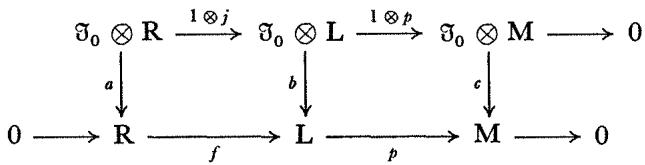
\includegraphics[keepaspectratio]{images/part003_24c814e1.jpg}}

其中 \(j\) 是典范单射， \(a, b, c\) 由典范单射 \(\mathfrak{I}_0 \to \mathbf{A}\) 导出（ \(\S 3\) , 第 4 号, 命题 4）；要证明的是 \(a\) 为满射。注意，由于 \(\mathbf{L}\) 是自由的， \(b\) 是单射的（ \(\S 3\) , 第 7 号, 命题 7 的推论 6），且 \(c\) 按假设是单射的。令 \(t\) 是 \(\mathbf{R}\) 的一个元素， \(t\) 是它在 \(\mathbf{R} / \mathfrak{I}_0\mathbf{R}\) 中的类；则有一个正合序列（ \(\S 3\) , 第 6 号, 命题 5 及命题 6 的推论 2）

\[
\mathrm{R} / \mathfrak {I} _ {0} \mathrm{R} \xrightarrow {\jmath} \mathrm{L} / \mathfrak {I} _ {0} \mathrm{L} \xrightarrow {\bar {p}} \mathrm{M} / \mathfrak {I} _ {0} \mathrm{M} \longrightarrow 0
\]

其中 \(j\) 和 \(\bar{p}\) 是 \(j\) 与 \(p\) 过渡到商时导出的，而 \(\bar{p}\) 按假设是双射；于是 \(\bar{j}(t) = 0\) ，换言之 \(j(t) \in \mathfrak{I}_0\mathbf{L}\) 。则存在一个元素 \(z \in \mathfrak{I}_0 \otimes \mathbf{L}\) 使得 \(j(t) = b(z)\) ；由于 \(p(b(z)) = 0\) ，有 \(c((1 \otimes p)(z)) = 0\) ，又由于 \(c\) 是单射，有 \((1 \otimes p)(z) = 0\) 。换言之， \(z\) 是某个元素 \(t' \in \mathfrak{I}_0 \otimes \mathbf{R}\) 在 \(1 \otimes j\) 下的像，于是 \(j(a(t')) = b(z) = j(t)\) ；由于 \(j\) 是单射，这就蕴含 \(t = a(t')\) 。

我们将在后文（交换代数, II, §3, 第 2 号, 命题 5）中说明如何把这命题推广到非分次模。

引理1. 交换群 \(\Delta\) 使得在 \(\Delta\) 上存在一个与 \(\Delta\) 的群结构相容的全序，其必要且充分的条件是 \(\Delta\) 无挠。

若在 \(\Delta\) 上存在这样一个序结构，且若 \(\lambda > 0\) ，则 \(\lambda + \mu > 0\) （对所有 \(\mu \geqslant 0\) ），特别地，对整数 \(n > 0\) 作归纳得 \(n.\lambda > 0\) ，这就证明 \(\Delta\) 是无挠的（因为每个元素 \(\neq 0\) （ \(\Delta\) 中的）或者 \(>0\) 或者 \(< 0\) ）。反之，若 \(\Delta\) 是无挠的，则 \(\Delta\) 是一个向量 \(\mathbf{Z}\) -空间的子 \(\mathbf{Q}\) -模（ \(\S 7\) , 第 10 号, 命题 26 的推论 1），可设它具有形式 \(\mathbf{Q}^{(I)}\) ；若给 I 一个良序（集合论, III, \(\S 2\) , 第 3 号, 定理 1），并给 \(\mathbf{Q}\) 其通常的序，则集合 \(\mathbf{Q}^{(I)}\) 赋予字典序是全序的（集合论, III, \(\S 2\) , 第 6 号）；立即看出这个序与 \(\mathbf{Q}^{(I)}\) 的加法群结构相容。

命题8. 设 \(\Delta\) 是一个无挠交换群，A 是一个类型为 \(\Delta\) 的分次环。若 A 中两个齐次元素 \(\neq 0\) 的乘积 \(\neq 0\) ，则环 A 没有零因子。

设 \(\Delta\) 被赋予与其群结构相容的全序（引理

\begin{enumerate}
\def\labelenumi{\arabic{enumi})}
\tightlist
\item
  ，并设 \(x = \sum_{\lambda \in \Delta} x_{\lambda}, y = \sum_{\lambda \in \Delta} y_{\lambda}\) 是 A 的两个非零元素（ \(x_{\lambda}\) 和 \(y_{\lambda}\) 是次数为 \(\lambda\) 的齐次元素，对所有 \(\lambda \in \Delta\) ）；设 \(\alpha\) （相应地， \(\beta\) ）是元素 \(\lambda \in \Delta\) （使 \(x_{\lambda} \neq 0\) （相应地， \(y_{\lambda} \neq 0\) ）者）中最大的；立即看出，若 \(\lambda \neq \alpha\) 或 \(\mu \neq \beta\) ，则或者 \(x_{\lambda}y_{\mu} = 0\) 或者 \(\deg(x_{\lambda}y_{\mu}) < \alpha + \beta\) ；因此 \(xy\) 的次数为 \(\alpha + \beta\) 的齐次分量是 \(x_{\alpha}y_{\beta}\) ，它按假设非零；从而 \(xy \neq 0\) 。
\end{enumerate}

\subsection{分次模的分次张量积}

设 \(\Delta\) 是一个交换幺半群，其单位元记作 0，A 是一个类型为 \(\Delta\) 的分次环，M（相应地，N）是一个类型为 \(\Delta\) 的分次右（相应地，左）A-模。设 \((\mathbf{A}_{\lambda})\) （相应地， \((\mathbf{M}_{\lambda}), (\mathbf{N}_{\lambda}))\) ）是 A（相应地，M，N）的分次；Z-模 M 和 N 的张量积 \(\mathbf{M} \otimes_{\mathbf{Z}} \mathbf{N}\) 是诸 \(\mathbf{M}_{\lambda} \otimes_{\mathbf{Z}} \mathbf{N}_{\mu}\) 的直和（§3, 第 7 号, 命题 7），因而后者构成这个 Z-模上类型为 \(\Delta, \Delta\) 的一个双分次。考虑 M \(\otimes_{\mathbf{Z}} \mathbf{N}\) 上与这个双分次相关联的类型为 \(\Delta\) 的全分次（第 1 号，例 4）；它由子 Z-模 \(\mathrm{P}_{\lambda} = \sum_{\mu + v = \lambda} (\mathrm{M}_{\mu} \otimes_{\mathbf{z}} \mathrm{N}_{v})\) 组成。已知 Z-模 M \(\otimes_{\mathbf{A}} \mathbf{N}\) 是 M \(\otimes_{\mathbf{Z}} \mathbf{N}\) 关于由元素 \((xa) \otimes y - x \otimes (ay)\) （其中 \(x \in \mathbf{M}, y \in \mathbf{N}\) 和 \(a \in \mathbf{A}\) ，§3, 第 1 号）生成的子 Z-模 Q 的商；如果对所有 \(\lambda \in \Delta\) , \(x_{\lambda}, y_{\lambda}, a_{\lambda}\) 分别是次数为 \(\lambda\) 的齐次分量（ \(x, y, a\) 的），则显然 \((xa) \otimes y - x \otimes (zy)\) 是齐次元素 \((x_{\lambda}a_{v}) \otimes y_{\mu} - x_{\lambda} \otimes (a_{v}y_{\mu})\) 之和，换言之，Q 是 M \(\otimes_{\mathbf{Z}} \mathbf{N}\) 的一个分次子 Z-模（第 3 号, 命题 2），且商

\[
\mathbf {M} \otimes_ {\mathbf {A}} \mathbf {N} = (\mathbf {M} \otimes_ {\mathbf {Z}} \mathbf {N}) / \mathbf {Q}
\]

因此典范地具有一个类型为 \(\Delta\) 的分次 Z-模结构（第 3 号）。此外（第 3 号, 命题 5），A 的中心 C 是 A 的一个分次子环；我们刚在 M \(\otimes_{\mathbf{A}} \mathbf{N}\) 上定义的这个分次与其在分次环 C 上的模结构相容。因为 M \(\otimes_{\mathbf{Z}} \mathbf{N}\) 典范地具有两个 C-模结构，对于它们分别有 \(c(x \otimes y) = (xc) \otimes y\) 和 \((x \otimes y)c = x \otimes (cy)\) （对 \(x \in \mathbf{M}, y \in \mathbf{N}, c \in \mathbf{C}\) ）（ \(\S 3\) , 第 3 号）；若 \(x \in \mathbf{M}_{\lambda}, y \in \mathbf{N}_{\mu}, c \in \mathbf{C} \cap \mathbf{A}_{\nu}\) ，则两个元素 \(c(x \otimes y)\) 和 \((x \otimes y)c\) 属于 (M \(\otimes_{\mathbf{Z}} \mathbf{N})_{\lambda + \mu + \nu}\) ，且它们的差属于 Q，因此它们在 M \(\otimes_{\mathbf{A}} \mathbf{N}\) 中的共同像属于 (M \(\otimes_{\mathbf{A}} \mathbf{N})_{\lambda + \mu + \nu}\) ，这便确立了我们的断言。当我们把 M \(\otimes_{\mathbf{A}} \mathbf{N}\) 作为分次 C-模谈论时，除非另有说明，总是指如此定义的结构。注意 (M \(\otimes_{\mathbf{A}} \mathbf{N})_{\lambda}\) 可以定义为 M \(\otimes_{\mathbf{A}} \mathbf{N}\) 的由诸 \(x_{\mu} \otimes y_{\nu}\) （其中 \(x_{\mu} \in \mathbf{M}_{\mu}, y_{\nu} \in \mathbf{N}_{\nu}\) 且 \(\mu + \nu = \lambda\) ）生成的加法子群。

设 \(\mathbf{M}'\) （相应地， \(\mathbf{N}'\) ）是另一个分次右（相应地，左）A-模，且 \(u: \mathbf{M} \to \mathbf{M}', v: \mathbf{N} \to \mathbf{N}'\) 是次数分别为 \(\alpha\) 和 \(\beta\) 的分次同态。那么由上述注记立即得出 \(u \otimes v\) 是次数为 \(\alpha + \beta\) 的分次（C-模）同态。

当A是交换环时，在任意有限多个分次A-模的张量积上同样可以定义与A-模结构相容的分次结构；此外，显然诸如结合性同构 \((\mathbf{M} \otimes \mathbf{N}) \otimes \mathbf{P} \to \mathbf{M} \otimes (\mathbf{N} \otimes \mathbf{P})\) (§ 3，第 8 号，命题 8)是分次模的同构。

注. 当 A 具有平凡分次（第 1 号，例 1）时， \((\mathbf{M} \otimes_{\mathbf{A}} \mathbf{N})_{\lambda}\) 就是诸子 Y-模 \(\mathbf{M}_{\mu} \otimes_{\mathbf{A}} \mathbf{N}_{\nu}\) （ \(\mathbf{M} \otimes_{\mathbf{A}} \mathbf{N}\) 中的，满足 \(\mu + \nu = \lambda\) ）的直和。

设 M（相应地，N）是类型为 \(\Delta\) 的分次右（相应地，左）A-模，P 是类型为 \(\Delta\) 的分次 Z-模，并设 f 是 \(M \times N\) 到 P 中的一个 Z-双线性映射，它满足 §3, 第 1 号的条件 (1)，且此外使得

\[
f (x _ {\lambda}, y _ {\mu}) \in \mathrm{P} _ {\lambda + \mu} \quad \text { for } x _ {\lambda} \in \mathrm{M} _ {\lambda}, y _ {\mu} \in \mathrm{N} _ {\mu}, \lambda , \mu \text { in } \Delta .
\]

那么 \(f(x, y) = g(x \otimes y)\) ，其中 \(g: \mathbf{M} \otimes_{\mathbf{A}} \mathbf{N} \to \mathbf{P}\) 是一个 \(\mathbf{Z}\) -线性映射（§3, 第 1 号, 命题 1），且由上述条件可知 \(g\) 是次数为 0 的分次 \(\mathbf{Z}\) -模同态。

设 B 是另一个类型为 \(\Delta\) 的分次环， \(\rho: A \to B\) 是分次环的一个同态（第 2 号）；则 \(\rho_*(B_d)\) 是类型为 \(\Delta\) 的一个分次右 A-模。若 E 是类型为 \(\Delta\) 的分次左 A-模，且给 \(\rho^*(B_d) \otimes_A E\) 赋予上面定义的类型为 \(\Delta\) 的分次 Z-模结构，则典范的左 B-模结构（ \(\S\) 5, 第 1 号）与

\[
\mathbf {E} _ {(\mathbf {B})} = \rho^ {*} (\mathbf {E}) = \rho_ {*} (\mathbf {B} _ {d}) \otimes_ {\mathbf {A}} \mathbf {E}.
\]

的分次相容。这样得到的分次 B-模称为借助 \(\rho\) 把纯量环扩张到 B 而得到的；当我们把 \(\mathrm{E}_{(\mathrm{B})}\) 或 \(\rho^{*}(\mathrm{E})\) 作为分次 B-模谈论时，除非另有说明，总是指这一结构。

\subsection{分次同态的分次模}

我们在本号中假设幺半群 \(\Delta\) 是一个群。设 A 是类型为 \(\Delta\) 的分次环，M、N 是两个类型为 \(\Delta\) 的分次左（例如）A-模。设 H \(_{\lambda}\) 表示由 M 到 N 的次数为 \(\lambda\) 的分次同态构成的加法群（第 2 号）；在 M 到 N 的所有同态（带非分次 A-模结构）的加法群 Hom \(_{A}\) (M, N) 中，对 \(\lambda \in \Delta\) 的诸 H \(_{\lambda}\) 之和是直和。因为，若有一个关系 \(\sum_{\lambda} u_{\lambda} = 0\) ，其中 \(u_{\lambda} \in \mathrm{H}_{\lambda}\) （对所有 \(\lambda\) ），则由此得出 \(\sum_{\lambda} u_{\lambda}(x_{\mu}) = 0\) （对所有 \(\mu\) 及所有 \(x_{\mu} \in \mathrm{M}_{\mu}\) ）。由于 \(\Delta\) 的元素都可消去， \(u_{\lambda}(x_{\mu})\) 是 \(\sum_{\lambda} u_{\lambda}(x_{\mu})\) 的次数为 \(\lambda + \mu\) 的齐次分量；因此 \(u_{\lambda}(x_{\mu}) = 0\) （对每个有序对 ( \(\mu, \lambda\) ) 及每个 \(x_{\mu} \in \mathrm{M}_{\mu}\) ），这蕴含 \(u_{\lambda} = 0\) （对所有 \(\lambda \in \Delta\) ）。我们（在本段中）用 Homgr \(_{A}\) (M, N) 表示 Hom \(_{A}\) (M, N) 的加法子群，即所有 H \(_{\lambda}\) 的和，并称之为从 M 到 N 的分次 A-模同态的加法群。设 C 为 A 的中心，它是一个分次子环（第 3 号，命题 5 的推论）；对于 \(\mathrm{Hom}_{\mathbf{A}}(\mathbf{M},\mathbf{N})\) 上的典范 C-模结构（§ 1，第 14 号，注记 1）， \(\mathrm{Homgr}_{\mathbf{A}}(\mathbf{M},\mathbf{N})\) 是一个子模，且分次 \((\mathbf{H}_{\lambda})\) 与 C-模结构相容：因为，若 \(c_{\nu}\in \mathbf{C}\cap \mathbf{A}_{\nu}\) , \(x_{\mu}\in \mathbf{N}_{\mu}\) 和 \(u_{\lambda}\in \mathbf{H}_{\lambda}\) ，则由定义 \((c_{\nu}u_{\lambda})(x_{\mu}) = c_{\nu}.u_{\lambda}(x_{\mu})\subset \mathbf{N}_{\lambda +\mu +\nu}\) ，因此 \(c_{\nu}u_{\lambda}\in \mathbf{H}_{\lambda +\nu}\) .

设 \(\mathbf{M}'\) 和 \(\mathbf{N}'\) 是两个类型为 \(\Delta\) 的分次左 A-模，且 \(u':\mathbf{M}'\to\mathbf{M}\) , \(v':\mathbf{N}\to\mathbf{N}'\) 是次数分别为 \(\alpha\) 和 \(\beta\) 的分次同态。那么立即看出 \(\operatorname{Hom}(u',v')\colon w\mapsto v'\circ w\circ u'\) 把 \(\operatorname{Homgr}_{\mathbf{A}}(\mathbf{M},\mathbf{N})\) 映到 \(\operatorname{Homgr}_{\mathbf{A}}(\mathbf{M}',\mathbf{N}')\) 中，且它到 \(\operatorname{Homgr}_{\mathbf{A}}(\mathbf{M},\mathbf{N})\) 的限制是到 \(\operatorname{Homgr}_{\mathbf{A}}(\mathbf{M}',\mathbf{N}')\) 中的次数为 \(\alpha+\beta\) 的分次同态。

特别地， \(\operatorname{Homgr}_{\mathbf{A}}(\mathbf{M}, \mathbf{M})\) 是 \(\operatorname{End}_{\mathbf{A}}(\mathbf{M})\) 的一个分次子环，记作 \(\operatorname{Endgr}_{\mathbf{A}}(\mathbf{M})\) 。

注. 若 M 和 N 是分次左 A-模， \(\operatorname{Homgr}_{\mathbf{A}}(\mathbf{M}, \mathbf{N})\) 一般不同于 \(\operatorname{Hom}_{\mathbf{A}}(\mathbf{M}, \mathbf{N})\) 。然而当 M 是有限生成的 A-模时，这两个集合相等。因为此时 M 由有限个齐次元素 \(x_{i}\) （ \(1 \leqslant i \leqslant n\) ）生成；设 \(d(i)\) 是 \(x_{i}\) 的次数；令 \(u \in \operatorname{Hom}_{\mathbf{A}}(\mathbf{M}, \mathbf{N})\) ，且对所有 \(\lambda \in \Delta\) ，设 \(z_{i,\lambda}\) 表示 \(u(x_{i})\) 的次数为 \(\lambda + d(i)\) 的齐次分量。我们证明存在一个同态 \(u_{\lambda}: \mathbf{M} \to \mathbf{N}\) ，使得 \(u_{\lambda}(x_{i}) = z_{i,\lambda}\) （对所有 \(i\) ）。只需证明若 \(\sum_{i} a_{i} x_{i} = 0\) ，其中 \(a_{i} \in \mathbf{A}\) （对于 \(1 \leqslant i \leqslant n\) ），则 \(\sum_{i} a_{i} z_{i,\lambda} = 0\) （对所有 \(\lambda \in \Delta\) ）（§1, 第 7 号, 注）。可以假设每个 \(a_{i}\) 都是次数为 \(d'(i)\) 的齐次元素，使得 \(d(i) + d'(i) = \mu\) （对所有 \(i\) ）（第 3 号, 注 1）；则 \(\sum_{i} a_{i} u(x_{i}) = 0\) ；在左边取次数为 \(\lambda + \mu\) 的齐次分量，我们得到 \(\sum_{i} a_{i} z_{i,\lambda} = 0\) ，由此得出同态 \(u_{\lambda}\) 的存在性；此外显然 \(u_{\lambda}\) 是次数为 \(\lambda\) 的分次同态。最后， \(u_{\lambda} = 0\) （除 \(\lambda\) 的有限多个值外），且按定义 \(u = \sum_{\lambda} u_{\lambda}\) ，这就证明了我们的断言。

特别地， \(\operatorname{Homgr}_{\mathbf{A}}(\mathbf{A}_s, \mathbf{M}) = \operatorname{Hom}_{\mathbf{A}}(\mathbf{A}_s, \mathbf{M})\) （对每个分次左 A-模 M）；此外 \(\operatorname{Hom}_{\mathbf{A}}(\mathbf{A}_s, \mathbf{M})\) 具有一个分次左 A-模结构（而不仅仅是分次 C-模结构），且显然在此结构下，M 到 \(\operatorname{Hom}_{\mathbf{A}}(\mathbf{A}_s, \mathbf{M})\) 中的典范映射（ \(\S 1\) , 第 14 号, 注 2）是一个分次 A-模同构。

类似地， \(\operatorname{Homgr}_{\mathbf{A}}(\mathbf{M}, \mathbf{A}_s)\) 具有一个分次右 A-模结构（而不仅仅是分次 C-模结构）；它称为分次 A-模 M 的分次对偶，记作 \(\mathbf{M}^{*\mathbf{gr}}\) ，或当不会引起混淆时简记作 \(\mathbf{M}^*\) 。如果 \(u: \mathbf{M} \to \mathbf{N}\) 是次数为 \(\delta\) 的分次同态，则由上述可知，到 \(\mathbf{N}^{*\mathbf{gr}}\) 上的 \(^t u = \operatorname{Hom}(u, 1_{\mathbf{A}_s})\) 的限制，是分次对偶 \(\mathbf{N}^{*\mathbf{gr}}\) 到分次对偶 \(\mathbf{M}^{*\mathbf{gr}}\) 中的一个次数为 \(\delta\) 的分次同态，称为 \(u\) 的分次转置。

我们有时在分次对偶 \(M^{*gr}\) 上考虑借助同构 \(\lambda\mapsto-\lambda\) （ \(\Delta\) 的）从上述分次导出的分次（第 1 号，例 2），使得次数为 \(\lambda\) 的齐次元素（ \(M^{*gr}\) 中的）是 M 上次数为 \(-\lambda\) 的分次线性形式（当 A 具有平凡分次时，这些是在 \(M_{\mu}\) （指标 \(\mu\neq\lambda\) 的）上为零的线性形式）。那么，若 \(u:M\to N\) 是次数为 \(\delta\) 的分次同态，则 \(u'\) 成为次数为 \(-\delta\) 的分次同态。

设 A 是交换的且类型为 \(\Delta\) 的分次环，且设 M、N、P、Q 是四个类型为 \(\Delta\) 的分次 A-模。则存在次数为 0 的典范分次同态

\begin{enumerate}
\def\labelenumi{(\arabic{enumi})}
\setcounter{enumi}{2}
\tightlist
\item
\end{enumerate}

\[
\operatorname{Homgr} _ {\mathbf {A}} (\mathbf {M}, \operatorname{Homgr} _ {\mathbf {A}} (\mathbf {N}, \mathbf {P})) \rightarrow \operatorname{Homgr} _ {\mathbf {A}} (\mathbf {M} \otimes_ {\mathbf {A}} \mathbf {N}, \mathbf {P})\tag{4}
\]

\[
\operatorname{Homgr} _ {\mathbf {A}} (\mathbf {M}, \mathbf {N}) \otimes_ {\mathbf {A}} \mathrm{P} \rightarrow \operatorname{Homgr} _ {\mathbf {A}} (\mathbf {M}, \mathbf {N} \otimes_ {\mathbf {A}} \mathrm{P})
\]

\[
\operatorname{Homgr} _ {\mathbf {A}} (\mathbf {M}, \mathbf {P}) \otimes_ {\mathbf {A}} \operatorname{Homgr} _ {\mathbf {A}} (\mathbf {N}, \mathbf {Q}) \rightarrow \operatorname{Homgr} _ {\mathbf {A}} (\mathbf {M} \otimes_ {\mathbf {A}} \mathbf {N}, \mathbf {P} \otimes_ {\mathbf {A}} \mathbf {Q}) \tag {5}
\]

（张量积赋予第 5 号中所定义的分次），它们由限制 §4, 第 1、2、4 号中所定义的典范同态而得到；事实上，若 \(u: \mathbf{M} \to \operatorname{Homgr}_{\mathbf{A}}(\mathbf{N}, \mathbf{P})\) 是次数为 \(\delta\) 的分次同态，那么对所有 \(x \in \mathbf{M}_{\lambda}\) , \(u(x)\) 是 \(\mathbf{N} \to \mathbf{P}\) 的次数为 \(\delta + \lambda\) 的分次同态，因此对于 \(y \in \mathbf{N}_{\mu}\) , \(u(x)(y) \in \mathbf{P}_{\delta + \lambda + \mu}\) ；若 \(v: \mathbf{M} \otimes_{\mathbf{A}} \mathbf{N} \to \mathbf{P}\) 典范地对应于 \(u\) ，则于是看出 \(v\) 是次数为 \(\delta\) 的分次同态，由此得出关于 (3) 的断言；此外还可看出这个同态是双射。对 (4) 和 (5) 的论证类似。

特别地，若 \(\mathbf{P} = \mathbf{Q} = \mathbf{A}\) 在(5)中，则存在一个次数为0的典范分次同态

\[
\mathbf {M} ^ {* \mathrm{gr}} \otimes_ {\mathbf {A}} \mathbf {N} ^ {* \mathrm{gr}} \rightarrow (\mathbf {M} \otimes_ {\mathbf {A}} \mathbf {N}) ^ {* \mathrm{gr}}.\tag{6}
\]

\BourbakiAppendixSection{伪模}

\subsection{向伪环添加单位元}

设 A 是一个伪环（I, §8, 第 1 号）。在集合 \(\mathbf{A}' = \mathbf{Z} \times \mathbf{A}\) 上，我们定义以下合成律：

\[
\left\{ \begin{array}{l} (m, a) + (n, b) = (m + n, a + b) \\ (m, a) (n, b) = (m n, m b + n a + a b). \end{array} \right.\tag{1}
\]

立即验证可知，A' 带这两个合成律是一个环，其中元素 \((1,0)\) 是单位元。集合 \(\{0\} \times A\) 是 A' 的一个双边理想，且 \(\iota: x \mapsto (0, x)\) 是伪环 A 到子伪环 \(\{0\} \times A\) 上的一个同构，借助它，A 与 \(\{0\} \times A\) 等同。A' 称为由伪环 A 添加单位元而导出的环。

如果 A 已经有一个单位元 \(\varepsilon\) ，则元素 \(e = (0, \varepsilon)\) （ \(\mathbf{A}'\) 中的）是属于 \(\mathbf{A}'\) 的中心的一个幂等元，且使得

\[
\mathrm{A} = e \mathrm{A} ^ {\prime} = \mathrm{A} ^ {\prime} e.
\]

则 \((e\mathbf{A}', (1 - e)\mathbf{A}')\) 是（I, §8, 第 11 号意义下的） \(\mathbf{A}'\) 的一个直和分解，且环 \((1 - e)\mathbf{A}'\) 同构于 \(\mathbf{Z}\) 。

\subsection{伪模}

给定一个含或不含单位元的伪环 A，A 上的左伪模是一个交换群 E（加法记法），它以 A 为算子集，且满足 §1, 第 1 号, 定义 1 的公理 \((\mathbf{M}_{\mathrm{I}})\) , \((\mathbf{M}_{\mathrm{II}})\) 和 \((\mathbf{M}_{\mathrm{III}})\) 。A 上的右伪模类似地定义。

设 \(A'\) 是给 A 添加单位元所得的环。若 E 是 A 上的一个左伪模，则在 E 上关联一个左 \(A'\) -模结构，其方式是对所有 \(x \in E\) 及每个元素 \((n, a) \in A'\) ，写下

\[
(n, a). x = n x + a x.\tag{2}
\]

公理 \((\mathbf{M}_{\mathrm{I}})\) 到 \((\mathbf{M}_{\mathrm{IV}})\) （§1, 第 1 号, 定义 1 的）立即得到验证；此外，把这个模结构的算子集限制到 \(\{0\} \times A\) （与 A 等同）上，我们就在 E 上重新得到最初给定的伪模结构。

对于 E 的子集 M，要使 M 成为伪模 E 的带算子子群（此时诱导结构显然也是 A 上的左伪模结构），当且仅当 M 是相伴 A'-模 E 的子模，且此子 A'-模与伪模 M 相伴。进而，商 A'-模 E/M 与带算子商群 E/M 相伴，而后者显然是 A 上的伪模。

若 E、F 是 A 上的两个伪模，则带算子群同态 \(E \rightarrow F\) 与分别相伴于伪模 E 和 F 的 A'-模之间的 A'-线性映射 \(E \rightarrow F\) 完全相同。若 \((\mathbf{E}_{t})_{t \in I}\) 是 A 上的一族伪模，则带算子群 \(\prod_{i\in I}E\) 和 \(\bigoplus_{i\in I}E_{i}\) 是 A 上的伪模，且相伴的 A'-模分别是相伴 A'-模 \(E_{i}\) 的积与直和。对伪模的逆极限与直极限也有类似的结果。因此，A 上伪模的理论可以完全归结为 A'-模的理论。

\BourbakiExercisesHeading
